\documentclass[13pt]{article}
\usepackage{graphicx}
\usepackage[utf8]{vietnam}
\usepackage{float}
\usepackage{tikz}
\usetikzlibrary{calc}
\usepackage{comment}
\usepackage[paperheight=29.7cm, paperwidth=21cm, right=2cm, left=3cm, top=2cm, bottom=2.5cm]{geometry}
\usepackage{hyperref}
\usepackage{listings}
\usepackage{xcolor}
\usepackage{longtable}
\usepackage{array}
\usepackage{booktabs}
\usepackage{enumitem}
\usepackage{fancyhdr}
\usepackage{setspace}

\hypersetup{
    colorlinks=true,
    linkcolor=blue,
    urlcolor=blue,
    citecolor=blue
}

\lstdefinestyle{pythonstyle}{
    backgroundcolor=\color{gray!10},
    basicstyle=\ttfamily\small,
    breaklines=true,
    frame=single,
    numbers=left,
    numberstyle=\tiny\color{gray},
    keywordstyle=\color{blue}\bfseries,
    stringstyle=\color{red},
    commentstyle=\color{green!60!black},
    showstringspaces=false
}

\lstdefinestyle{sqlstyle}{
    backgroundcolor=\color{blue!5},
    basicstyle=\ttfamily\small,
    breaklines=true,
    frame=single,
    numbers=left,
    numberstyle=\tiny\color{gray},
    keywordstyle=\color{blue}\bfseries,
    stringstyle=\color{red},
    commentstyle=\color{green!60!black},
    showstringspaces=false,
    morekeywords={SELECT, FROM, WHERE, GROUP, BY, AS, CREATE, REPLACE, MODEL, OPTIONS, IF, LIMIT, AVG, COUNT}
}

\lstdefinestyle{shellstyle}{
    backgroundcolor=\color{black!5},
    basicstyle=\ttfamily\small,
    breaklines=true,
    frame=single,
    showstringspaces=false
}

\setstretch{1.15}

\begin{document}

%% ==================== BÌA ====================
\begin{titlepage}
\begin{tikzpicture}[overlay,remember picture]
\draw [line width=3pt]
    ($(current page.north west) + (3cm,-2cm)$)
    rectangle
    ($(current page.south east) + (-2cm,2.5cm)$);
\draw [line width=0.5pt]
    ($(current page.north west) + (3.1cm,-2.1cm)$)
    rectangle
    ($(current page.south east) + (-2.1cm,2.6cm)$);
\end{tikzpicture}
\begin{center}

\vspace{-6pt}
\textbf{\fontsize{14pt}{16pt}\selectfont
ĐẠI HỌC QUỐC GIA THÀNH PHỐ HỒ CHÍ MINH\\
TRƯỜNG ĐẠI HỌC KHOA HỌC TỰ NHIÊN\\
KHOA CÔNG NGHỆ THÔNG TIN}
\vspace{0.5cm}
\begin{figure}[H]
    \centering
    \includegraphics[scale=0.2]{image/KHTN.png}
\end{figure}

\vspace{1cm}
\fontsize{14pt}{16pt}\selectfont NHẬP MÔN ĐIỆN TOÁN ĐÁM MÂY -- CSC11006\\
ĐỒ ÁN SỐ 1\\
\vspace{12pt}
\textbf{\fontsize{18pt}{20pt}\selectfont INTELLIGENT CLOUD-BASED}\\
\textbf{\fontsize{18pt}{20pt}\selectfont LOG ANALYTICS \& BI SYSTEM}

\vspace{0.5cm}
\fontsize{12pt}{14pt}\selectfont
\textit{Hệ Thống Phân Tích Log Thông Minh Trên Nền Tảng Đám Mây}

\vspace{2cm}
\begin{tabular}{l l}
    \fontsize{13pt}{15pt}\selectfont Sinh viên thực hiện: & \fontsize{13pt}{15pt}\selectfont Trương Nhật Đạt -- 23120231 \\
    & \fontsize{13pt}{15pt}\selectfont Ngô Gia An -- 23120205 \\
    & \fontsize{13pt}{15pt}\selectfont Nguyễn Văn Bình Dương -- 23120242 \\
    & \\
    \fontsize{13pt}{15pt}\selectfont Giảng viên hướng dẫn: & \fontsize{13pt}{15pt}\selectfont Cô Chung Thuỳ Linh \\
    & \fontsize{13pt}{15pt}\selectfont Thầy Lê Ngọc Sơn \\
\end{tabular}

\vspace{2.5cm}
\fontsize{13pt}{15pt}\selectfont Thành Phố Hồ Chí Minh, tháng 5 năm 2026
\end{center}
\end{titlepage}

\newpage
\tableofcontents
\newpage

%% ==================== PHẦN 1 ====================
\section{Đánh giá Mức độ Hoàn thành}
\subsection{Phân công công việc và Đóng góp}
Dự án được thực hiện bởi nhóm 3 thành viên, với sự phân chia công việc rõ ràng và tỷ lệ đóng góp đồng đều:
\begin{itemize}
    \item \textbf{Thành viên A:} Nguyễn Văn Bình Dương -- 23120242 (33.3\%) -- Phụ trách thiết kế và phát triển Frontend, triển khai S3 \& CloudFront, và tích hợp Cognito.
    \item \textbf{Thành viên B:} Ngô Gia An -- 23120205 (33.3\%) -- Phụ trách Backend API (Lambda), cơ sở dữ liệu DynamoDB, API Gateway, luồng Request.
    \item \textbf{Thành viên C:} Trương Nhật Đạt -- 23120231 (33.3\%) -- Phụ trách hạ tầng VPC, bảo mật IAM, hệ thống giám sát CloudWatch, quản lý chi phí.
\end{itemize}

\subsection{Danh mục hình ảnh minh chứng}
Bảng dưới đây tổng hợp các ký hiệu hình ảnh minh chứng theo yêu cầu của đồ án, ý nghĩa của từng ảnh và đường dẫn (link) để nhảy nhanh đến ảnh tương ứng trong báo cáo:

\begin{longtable}{|p{0.15\textwidth}|p{0.6\textwidth}|p{0.15\textwidth}|}
\hline
\textbf{Ký hiệu} & \textbf{Ý nghĩa minh chứng} & \textbf{Đường dẫn} \\ \hline
\endfirsthead
\hline
\textbf{Ký hiệu} & \textbf{Ý nghĩa minh chứng} & \textbf{Đường dẫn} \\ \hline
\endhead
SE-1 & S3 Bucket Block Public Access bật 4 tùy chọn & \hyperref[img:SE-1]{Xem ảnh} \\ \hline
SE-2 & Truy cập trực tiếp S3 bị cấm (403 Forbidden) & \hyperref[img:SE-2]{Xem ảnh} \\ \hline
SE-3 & Truy cập thông qua CloudFront thành công (200 OK) & \hyperref[img:SE-3]{Xem ảnh} \\ \hline
SE-4 & Cấu hình Origin Access Control (OAC) & \hyperref[img:SE-4]{Xem ảnh} \\ \hline
NE-1 & VPC Gateway Endpoint cho DynamoDB (Available) & \hyperref[img:NE-1]{Xem ảnh} \\ \hline
NE-2 & Cấu hình Lambda trong Custom VPC & \hyperref[img:NE-2.1]{Xem ảnh} \\ \hline
NE-3 & Route Table có dòng điều hướng qua VPCE & \hyperref[img:NE-3]{Xem ảnh} \\ \hline
NE-4 & Không sử dụng NAT Gateway (Trống/Deleted) & \hyperref[img:NE-4]{Xem ảnh} \\ \hline
NE-5 & CloudWatch Log gọi DynamoDB thành công & \hyperref[img:NE-5.1]{Xem ảnh} \\ \hline
IM-1 & Các IAM Roles được phân chia riêng biệt cho từng Lambda & \hyperref[img:IM-1]{Xem ảnh} \\ \hline
IM-2 & Policy giới hạn quyền trên ARN cụ thể (Không dùng *) & \hyperref[img:IM-2.1]{Xem ảnh} \\ \hline
IM-3 & Gắn đúng IAM Role cho từng Lambda Function & \hyperref[img:IM-3.1]{Xem ảnh} \\ \hline
CO-2 & Cấu hình Cognito Authorizer trên API Gateway & \hyperref[img:CO-2]{Xem ảnh} \\ \hline
CO-3 & Gọi API bị chặn nếu không có Token & \hyperref[img:CO-3]{Xem ảnh} \\ \hline
CO-4 & Gọi API thành công khi có Token hợp lệ & \hyperref[img:CO-4.1]{Xem ảnh} \\ \hline
DB-1 & CloudWatch Dashboard theo dõi hệ thống & \hyperref[img:DB-1]{Xem ảnh} \\ \hline
CW-1 & CloudWatch Alarms giám sát lỗi & \hyperref[img:CW-1]{Xem ảnh} \\ \hline
BG-1 & Cấu hình AWS Budget giới hạn chi phí & \hyperref[img:BG-1]{Xem ảnh} \\ \hline
CS-1 & Báo cáo Cost Explorer chứng minh chi phí \$0 & \hyperref[img:CS-1]{Xem ảnh} \\ \hline
SD-1 & Sơ đồ so sánh VPC Gateway Endpoint vs NAT Gateway & \hyperref[img:SD-1]{Xem ảnh} \\ \hline
SD-2 & Sơ đồ kiến trúc Serverless hệ thống tổng thể & \hyperref[img:SD-2]{Xem ảnh} \\ \hline
SD-3 & Sơ đồ tuần tự luồng Request & \hyperref[img:SD-3]{Xem ảnh} \\ \hline
\end{longtable}
\newpage

%% ==================== PHẦN 1 ====================
\section{Thiết kế và Phát triển Frontend}

\subsection{Công nghệ sử dụng}
Giao diện ứng dụng Task Manager được phát triển bằng bộ ba công nghệ web cơ bản: \textbf{HTML5, CSS3 và JavaScript thuần (Vanilla JS)}, không sử dụng bất kỳ framework frontend nào như React, Angular hay Vue. Lựa chọn này hoàn toàn phù hợp với yêu cầu đề bài và mang lại hai lợi thế rõ rệt:

\begin{itemize}
    \item \textbf{Nhẹ và nhanh:} Toàn bộ mã nguồn frontend chỉ bao gồm các file tĩnh (HTML, CSS, JS) có tổng dung lượng rất nhỏ (dưới 50KB), hoàn hảo để đóng gói vào Amazon S3 và phân phối qua CloudFront.
    \item \textbf{Không phụ thuộc server-side rendering:} Do ứng dụng hoàn toàn là Static Website phía client, việc hosting trên S3 (với chế độ Private + CloudFront) trở nên cực kỳ đơn giản và tối ưu chi phí.
\end{itemize}

\textbf{Thư viện bên ngoài duy nhất được sử dụng:}
\begin{itemize}
    \item \textbf{amazon-cognito-identity-js} (tải qua CDN từ jsDelivr): Đây là thư viện chính thức của AWS dùng để tương tác với dịch vụ Amazon Cognito từ phía trình duyệt. Nó cung cấp các hàm đăng ký, đăng nhập, xác nhận OTP và quản lý phiên JWT Token.
    \item \textbf{Google Fonts -- Inter:} Font chữ hiện đại, dễ đọc, được sử dụng xuyên suốt giao diện.
\end{itemize}

\subsection{Các tính năng đã triển khai}

\subsubsection{Hệ thống xác thực người dùng (Authentication)}
Ứng dụng sử dụng \textbf{Amazon Cognito} để quản lý tài khoản. Luồng xác thực diễn ra hoàn toàn phía client:

\begin{longtable}{|p{0.2\textwidth}|p{0.75\textwidth}|}
\hline
\textbf{Chức năng} & \textbf{Mô tả chi tiết} \\ \hline
\endhead
\textbf{Đăng ký} & Người dùng nhập email và mật khẩu. Cognito gửi mã OTP 6 số về email để xác nhận. Sau khi nhập đúng mã, tài khoản được kích hoạt. \\ \hline
\textbf{Đăng nhập} & Cognito xác thực và trả về bộ 3 token (ID Token, Access Token, Refresh Token). Frontend lưu ID Token (JWT) vào \texttt{localStorage}. \\ \hline
\textbf{Đăng xuất} & Xóa token khỏi \texttt{localStorage}, hủy phiên trên Cognito, rồi chuyển hướng về trang Login. \\ \hline
\textbf{Bảo vệ trang} & Hàm \texttt{requireAuth()} kiểm tra xem JWT Token trong \texttt{localStorage} còn hạn hay không. Nếu hết hạn hoặc không có token, tự động redirect về Login. \\ \hline
\end{longtable}

\subsubsection{Quản lý công việc — CRUD đầy đủ}

\begin{longtable}{|p{0.2\textwidth}|p{0.75\textwidth}|}
\hline
\textbf{Thao tác} & \textbf{Mô tả} \\ \hline
\endhead
\textbf{Tạo mới (Create)} & Gọi \texttt{POST /tasks} gửi dữ liệu lên Lambda (Tiêu đề, Mô tả, Mức ưu tiên, Ngày hạn). \\ \hline
\textbf{Xem danh sách (Read)} & Gọi \texttt{GET /tasks} để lấy toàn bộ công việc của user đang đăng nhập. Danh sách hiển thị dạng card mã màu theo ưu tiên. \\ \hline
\textbf{Cập nhật (Update)} & Gọi \texttt{PUT /tasks/:id} cập nhật dữ liệu. Cho phép chuyển trạng thái \texttt{pending} sang \texttt{done}. \\ \hline
\textbf{Xóa (Delete)} & Hộp thoại xác nhận hiện ra. Nếu đồng ý, gọi \texttt{DELETE /tasks/:id}. \\ \hline
\end{longtable}

\subsubsection{Bộ lọc công việc}
Frontend triển khai bộ lọc kết hợp các tiêu chí:
\begin{itemize}
    \item \textbf{Lọc theo Mức ưu tiên (Priority):} Dropdown cho phép chọn Tất cả, Cao, Trung bình hoặc Thấp.
    \item \textbf{Lọc theo Khoảng ngày hạn (Date Range):} Hai trường ``Từ ngày'' và ``Đến ngày'' thu hẹp kết quả.
    \item \textbf{Kết hợp nhiều bộ lọc:} Có thể lọc đồng thời cả mức ưu tiên và khoảng ngày hạn. Bộ lọc hoạt động hoàn toàn phía client.
\end{itemize}

\subsection{Triển khai Frontend trên AWS (S3 Private + CloudFront + OAC)}

Thay vì để S3 bucket ở chế độ Public, nhóm triển khai mô hình bảo mật theo yêu cầu:

\begin{figure}[H]
    \centering
    \begin{tikzpicture}[node distance=2cm]
        \node (user) [draw, rectangle, minimum width=2cm, minimum height=1cm] {Người dùng};
        \node (cf) [draw, rectangle, below of=user, minimum width=2cm, minimum height=1cm] {CloudFront CDN};
        \node (s3) [draw, rectangle, below of=cf, minimum width=2cm, minimum height=1cm] {S3 Bucket (PRIVATE)};
        \node (oac) [right of=cf, node distance=4cm] {Origin Access Control};
        
        \draw[->, thick] (user) -- (cf);
        \draw[->, thick] (cf) -- (s3);
        \draw[<->, dashed] (cf) -- (oac);
    \end{tikzpicture}
    \caption{Luồng phân phối Frontend}
\end{figure}

S3 bucket được cấu hình hoàn toàn \textbf{PRIVATE} — tất cả 4 tùy chọn Block Public Access đều BẬT. Không ai có thể truy cập file trực tiếp qua URL S3 (sẽ nhận lỗi 403 Forbidden). Chỉ duy nhất CloudFront (thông qua OAC) mới được phép đọc file từ bucket.

\begin{figure}[H]
    \centering
    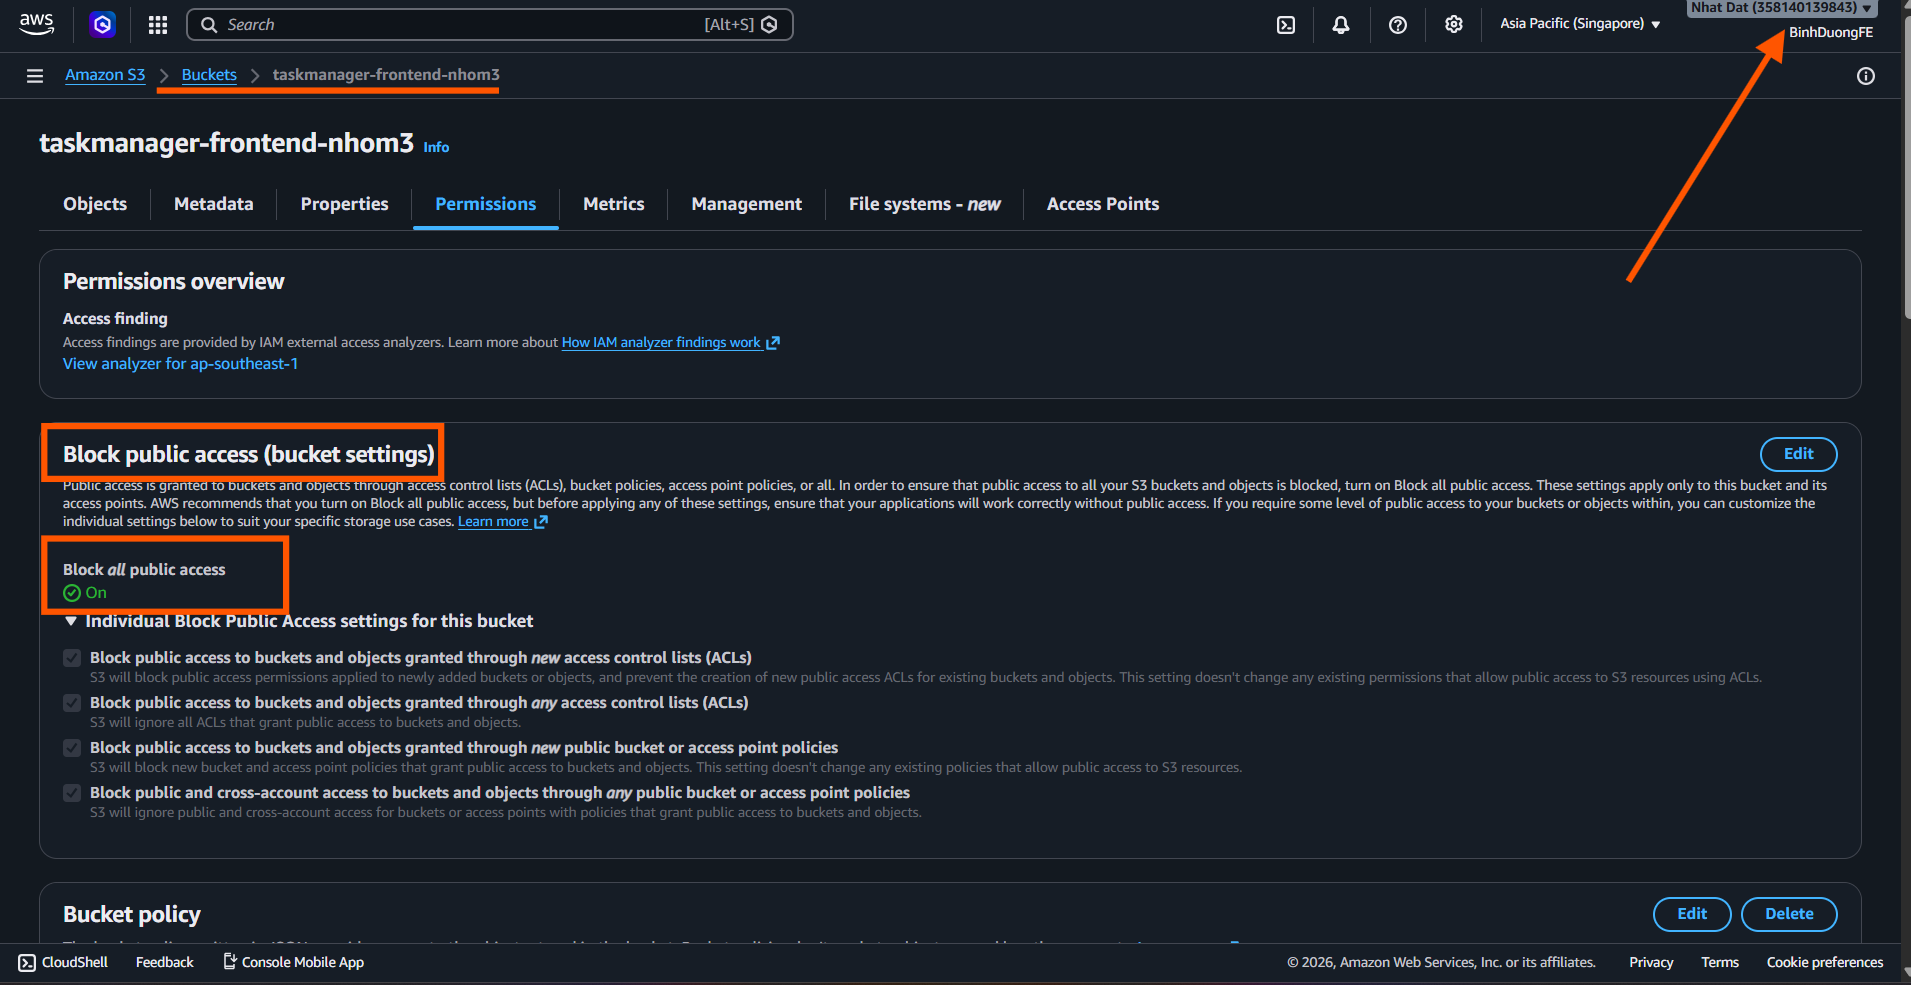
\includegraphics[width=0.8\textwidth]{image/SE-1.png}
    \caption{SE-1: S3 Bucket Block Public Access}
    \label{img:SE-1}
\end{figure}

\begin{figure}[H]
    \centering
    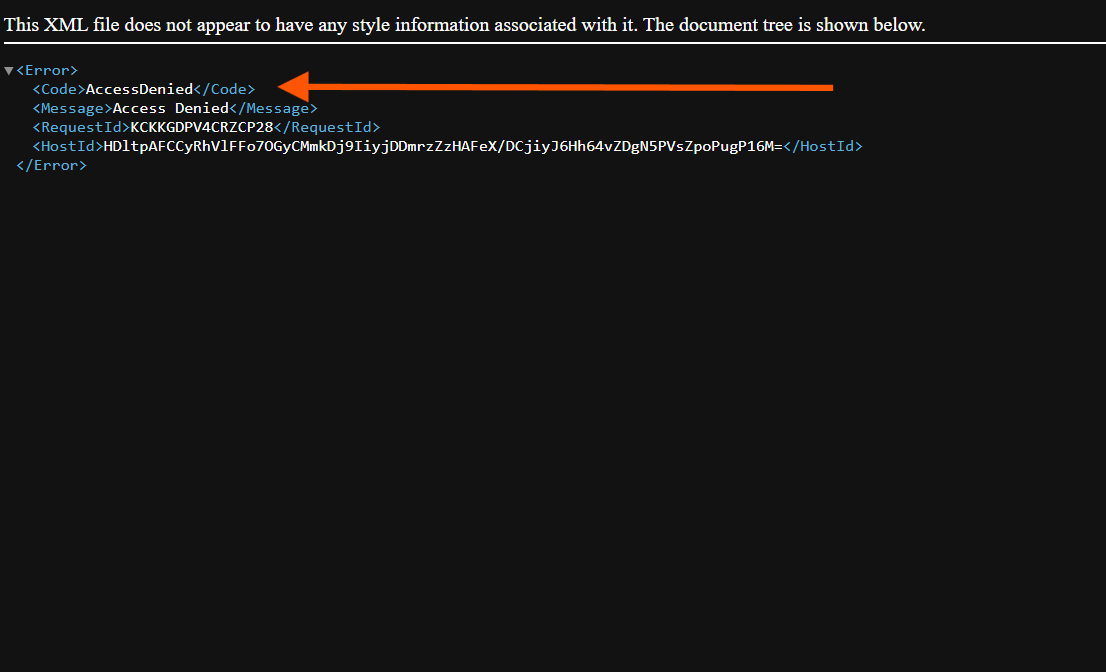
\includegraphics[width=0.8\textwidth]{image/SE-2.png}
    \caption{SE-2: Truy cập trực tiếp S3 bị cấm (403 Forbidden)}
    \label{img:SE-2}
\end{figure}

\begin{figure}[H]
    \centering
    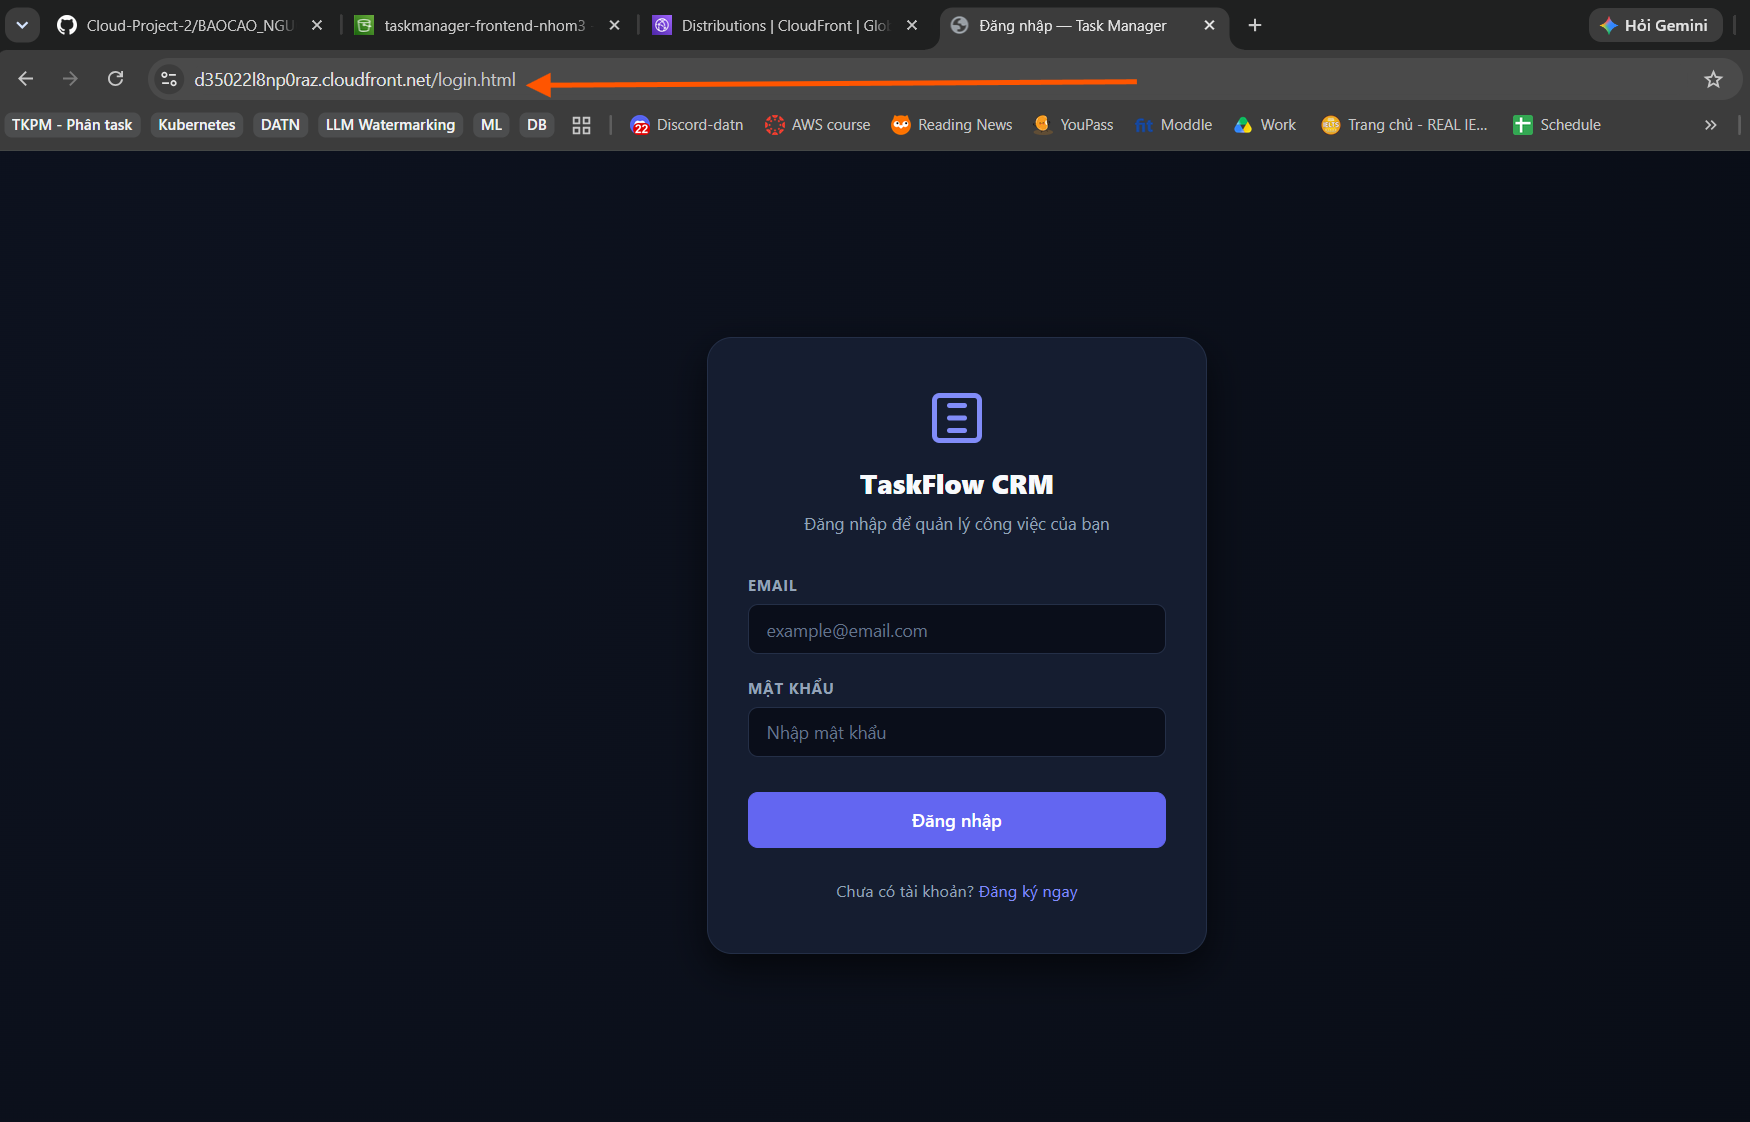
\includegraphics[width=0.8\textwidth]{image/SE-3.png}
    \caption{SE-3: Truy cập thông qua CloudFront thành công}
    \label{img:SE-3}
\end{figure}

\begin{figure}[H]
    \centering
    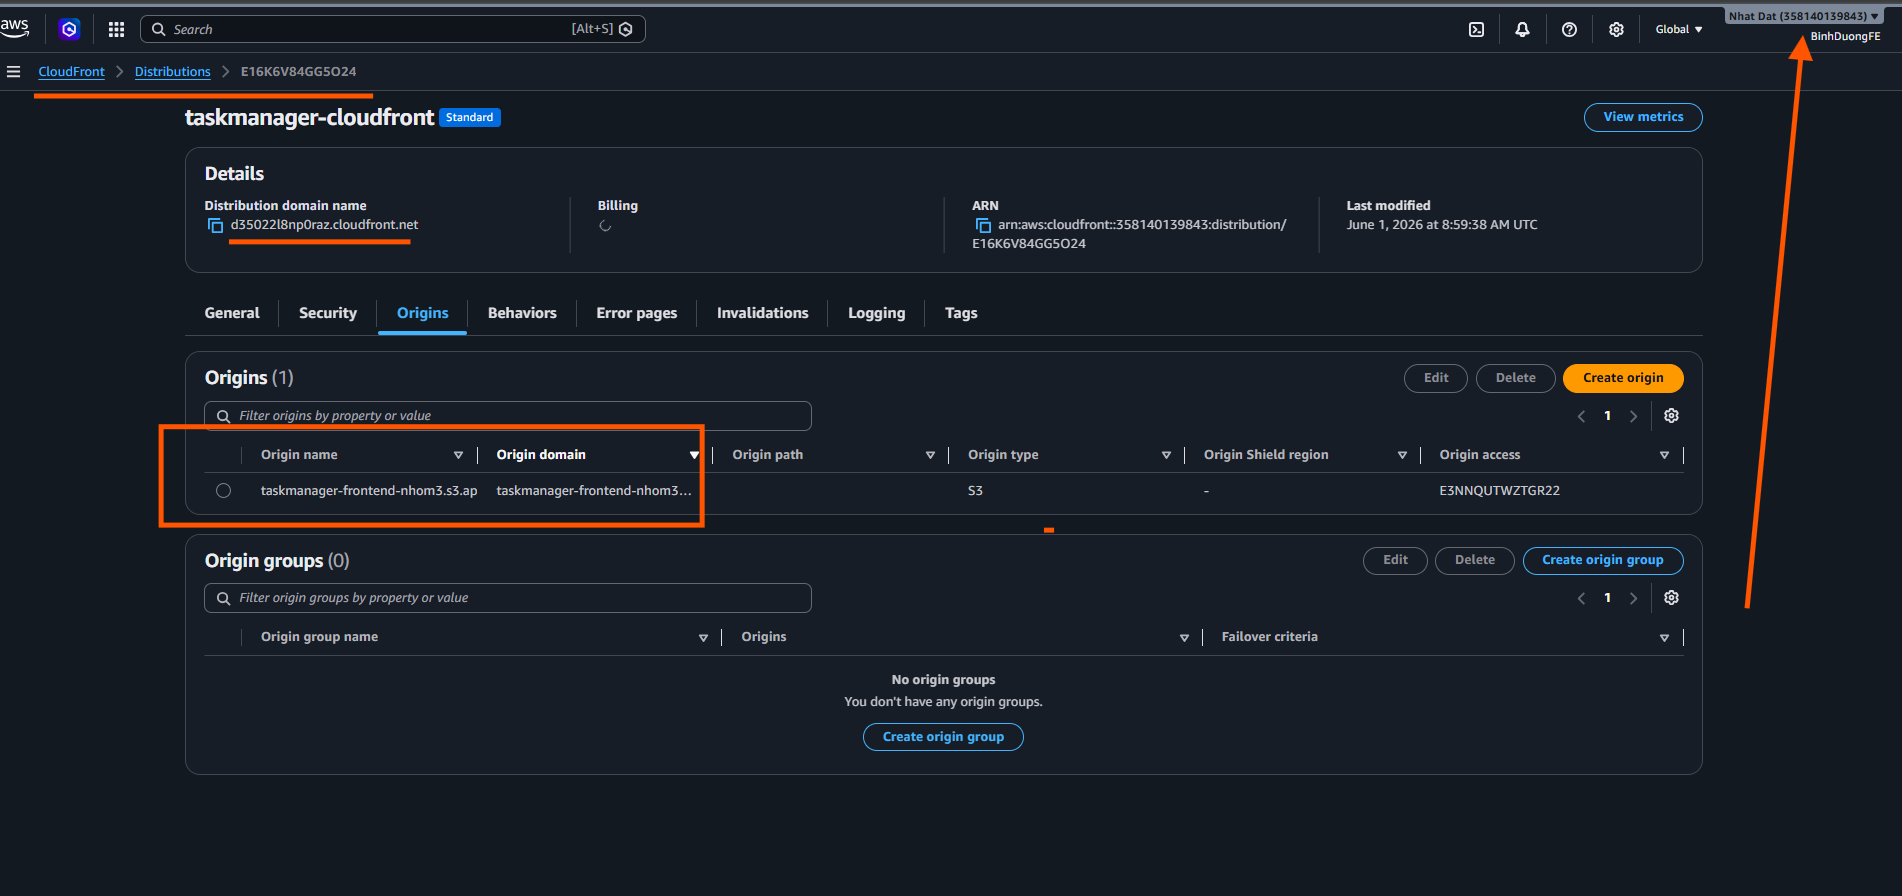
\includegraphics[width=0.8\textwidth]{image/SE-4.png}
    \caption{SE-4: Cấu hình Origin Access Control (OAC)}
    \label{img:SE-4}
\end{figure}


%% ==================== PHẦN 2 ====================
\section{Thiết kế Backend API và Cơ sở Dữ liệu}

\subsection{Kiến trúc 4 Lambda Functions riêng biệt}
Backend sử dụng Node.js 22.x, hệ thống gồm 4 hàm Lambda độc lập, mỗi hàm đảm nhận đúng một chức năng CRUD:

\begin{longtable}{|p{0.3\textwidth}|p{0.15\textwidth}|p{0.5\textwidth}|}
\hline
\textbf{Lambda Function} & \textbf{Method} & \textbf{Chức năng chính} \\ \hline
\endhead
\texttt{TaskManager-GetTasks} & GET & Lấy danh sách công việc của user đang đăng nhập (dùng Query trên GSI) \\ \hline
\texttt{TaskManager-CreateTask} & POST & Tạo công việc mới (PutItem) \\ \hline
\texttt{TaskManager-UpdateTask} & PUT & Cập nhật nội dung công việc (UpdateItem với ConditionExpression) \\ \hline
\texttt{TaskManager-DeleteTask} & DELETE & Xóa công việc (DeleteItem) \\ \hline
\end{longtable}

Cả 4 Lambda đều được đặt vào trong Custom VPC nhằm đảm bảo kết nối đến DynamoDB đi qua VPC Gateway Endpoint (mạng riêng của AWS) thay vì internet công cộng.

\begin{figure}[H]
    \centering
    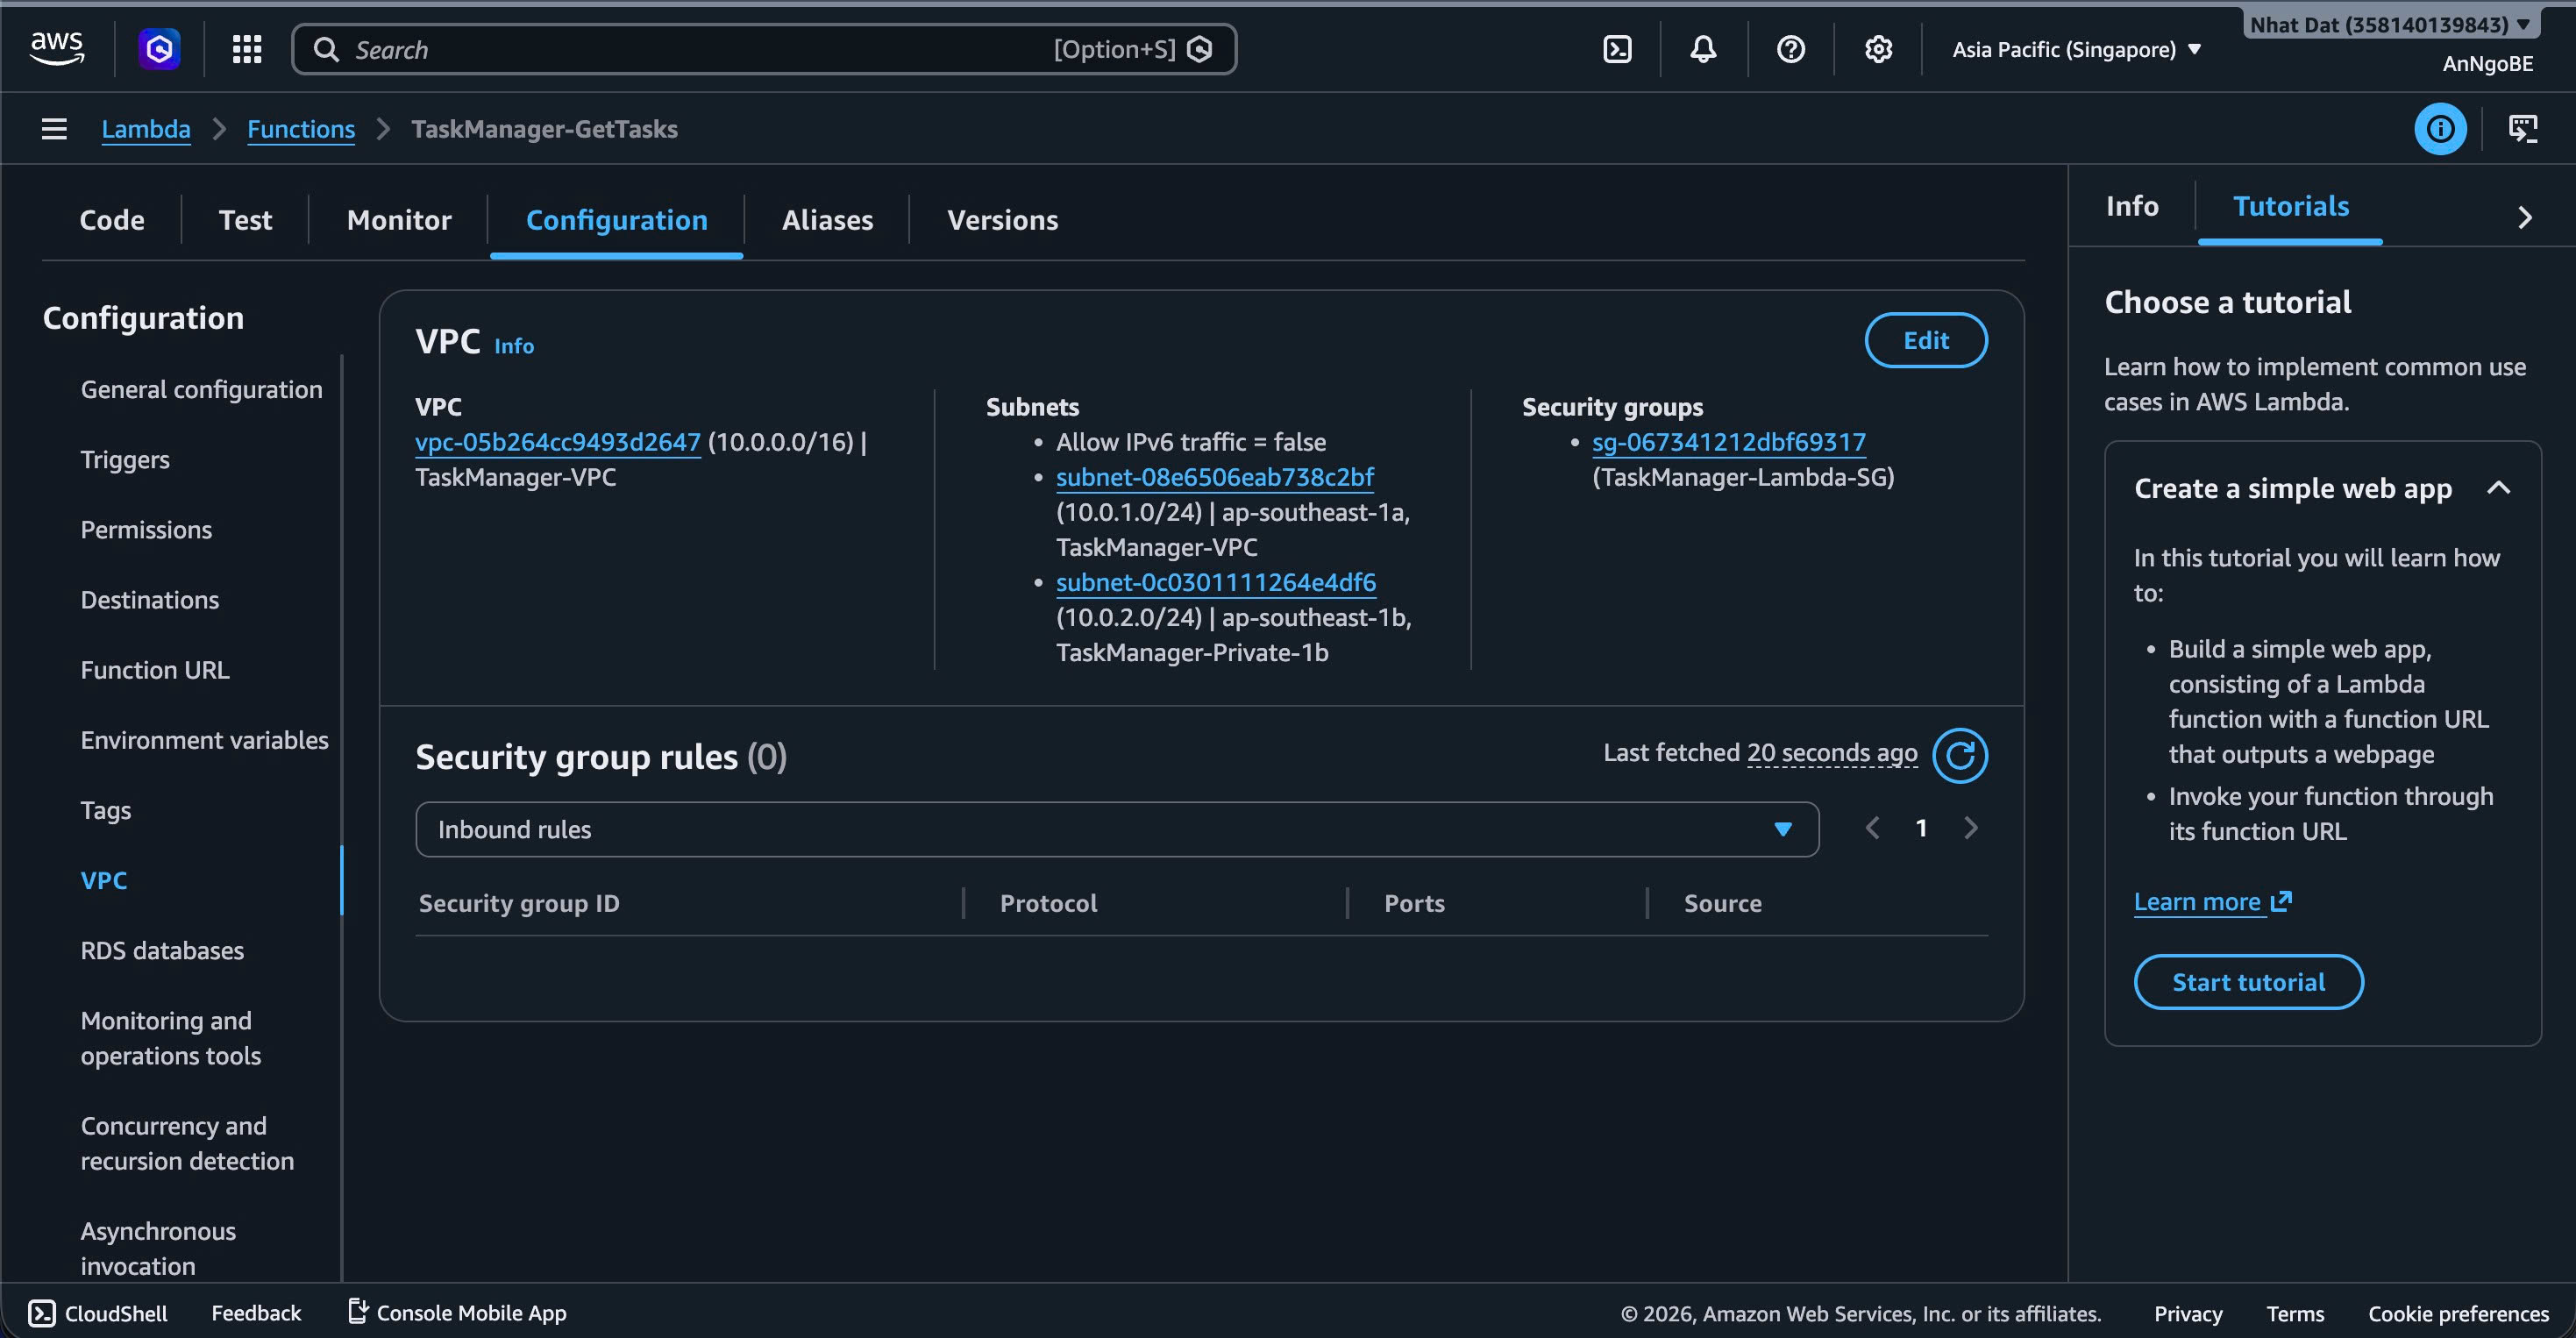
\includegraphics[width=0.8\textwidth]{image/NE-2.1.jpg}
    \caption{NE-2: Cấu hình VPC cho Lambda GetTasks}
    \label{img:NE-2.1}
\end{figure}

\subsection{Cơ sở Dữ liệu Amazon DynamoDB}
Amazon DynamoDB được chọn vì hoàn toàn serverless, không cần quản trị server, High Availability tích hợp sẵn, và Free Tier rộng rãi.

\textbf{Schema bảng dữ liệu (TasksTable):}
\begin{itemize}
    \item \texttt{taskId} (String): \textbf{Partition Key}. Chuỗi UUID duy nhất.
    \item \texttt{userId} (String): \textbf{GSI Partition Key}. Là \texttt{sub} claim từ Cognito.
    \item Các thuộc tính khác: \texttt{title}, \texttt{description}, \texttt{priority}, \texttt{dueDate}, \texttt{status}, \texttt{createdAt}.
\end{itemize}

\textbf{Global Secondary Index (GSI):} 
GSI \texttt{userId-index} được tạo với Partition Key là \texttt{userId}. GSI này cho phép hàm GetTasks thực hiện Query cực kỳ hiệu quả để trả về tất cả bản ghi có \texttt{userId = X} thay vì phải Scan toàn bộ bảng.

\subsection{API Gateway — Định tuyến và Bảo mật}
API Gateway (REST API) được sử dụng để điều hướng các request đến các hàm Lambda tương ứng.

\begin{figure}[H]
    \centering
    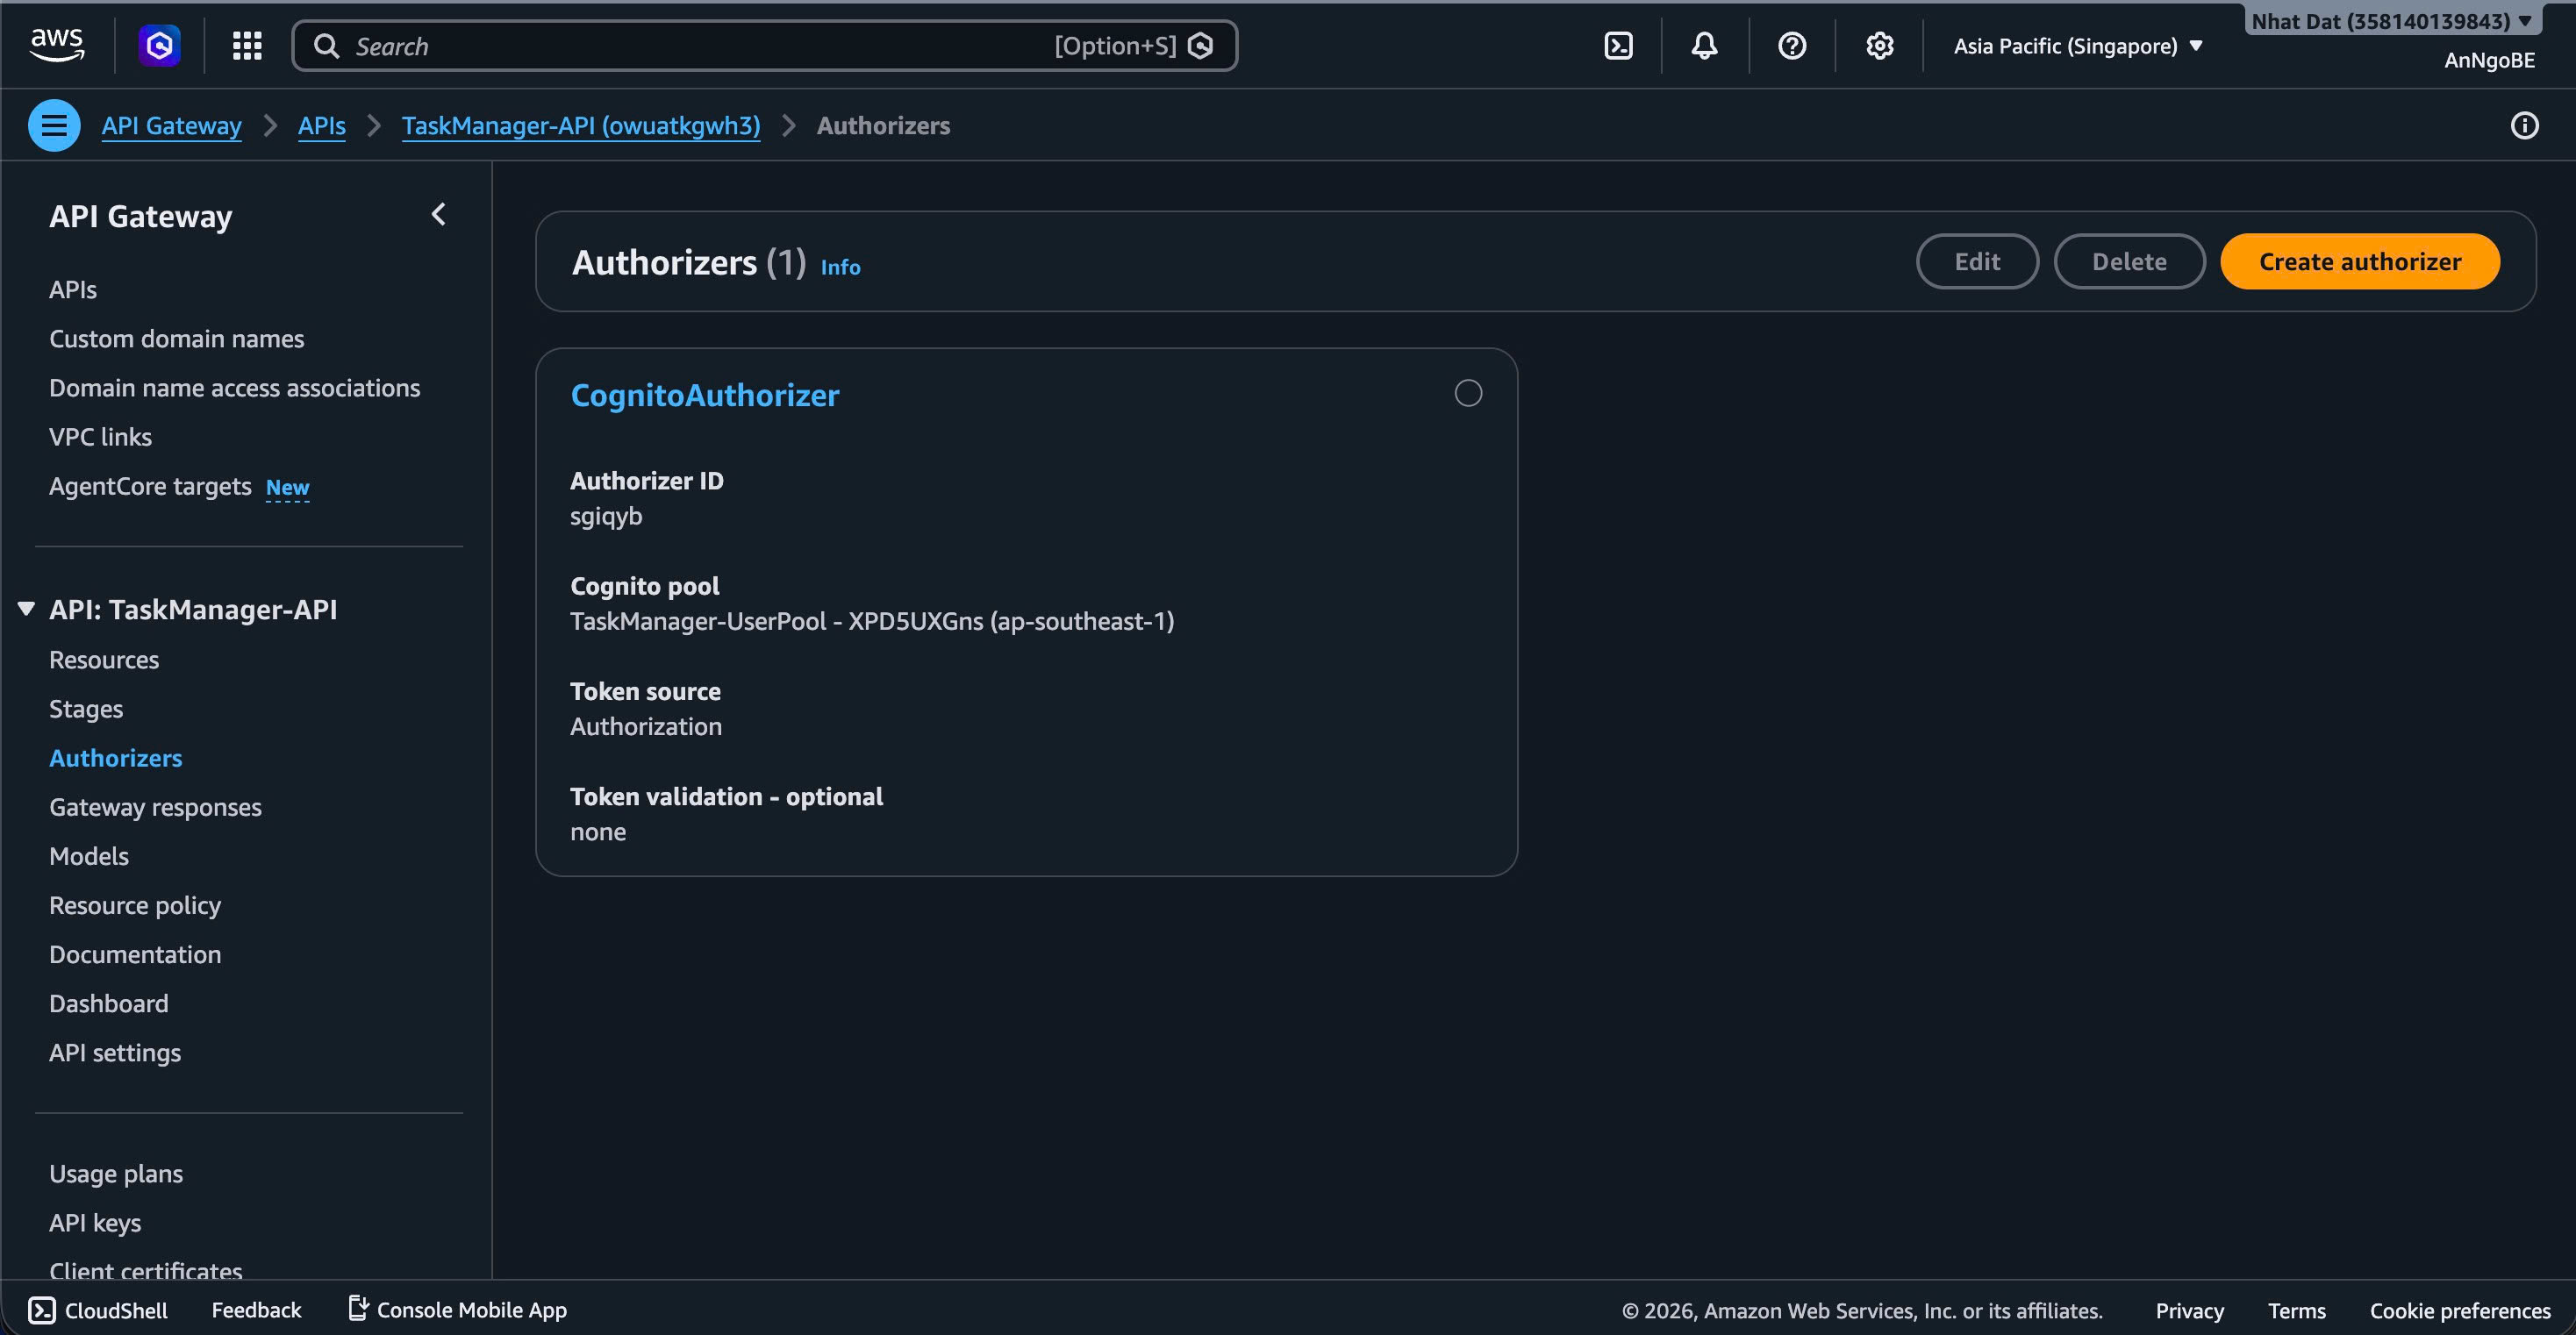
\includegraphics[width=0.8\textwidth]{image/CO-2.jpg}
    \caption{CO-2: Cấu hình Cognito Authorizer trên API Gateway}
    \label{img:CO-2}
\end{figure}

\textbf{Cognito Authorizer:} 
API Gateway tự động giải mã và xác minh JWT Token trong header Authorization. Nếu hợp lệ, cho phép request đi tiếp vào Lambda. Nếu không hợp lệ, trả về 401 Unauthorized ngay lập tức.

\begin{figure}[H]
    \centering
    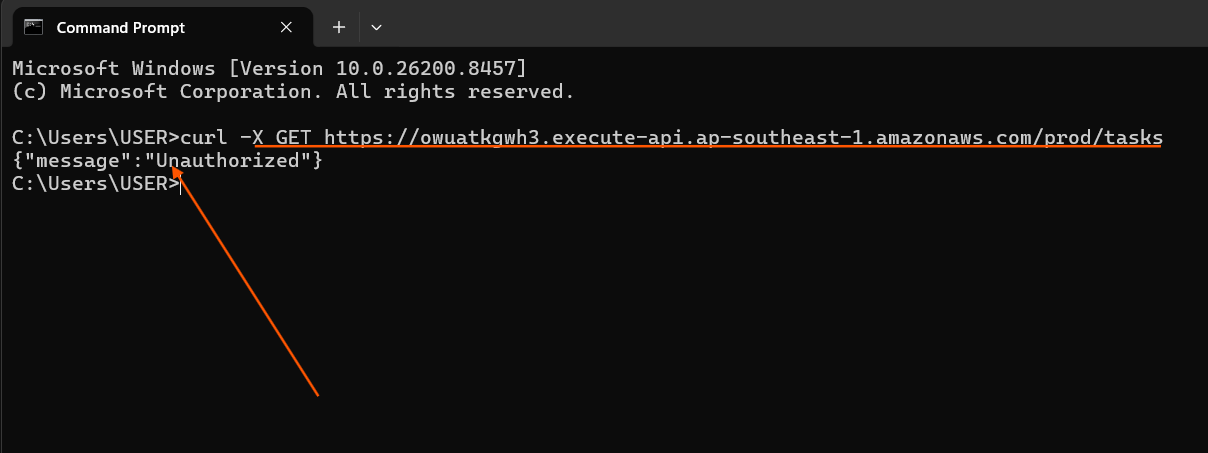
\includegraphics[width=0.8\textwidth]{image/CO-3.png}
    \caption{CO-3: Gọi API không có Token (401 Unauthorized)}
    \label{img:CO-3}
\end{figure}

\begin{figure}[H]
    \centering
    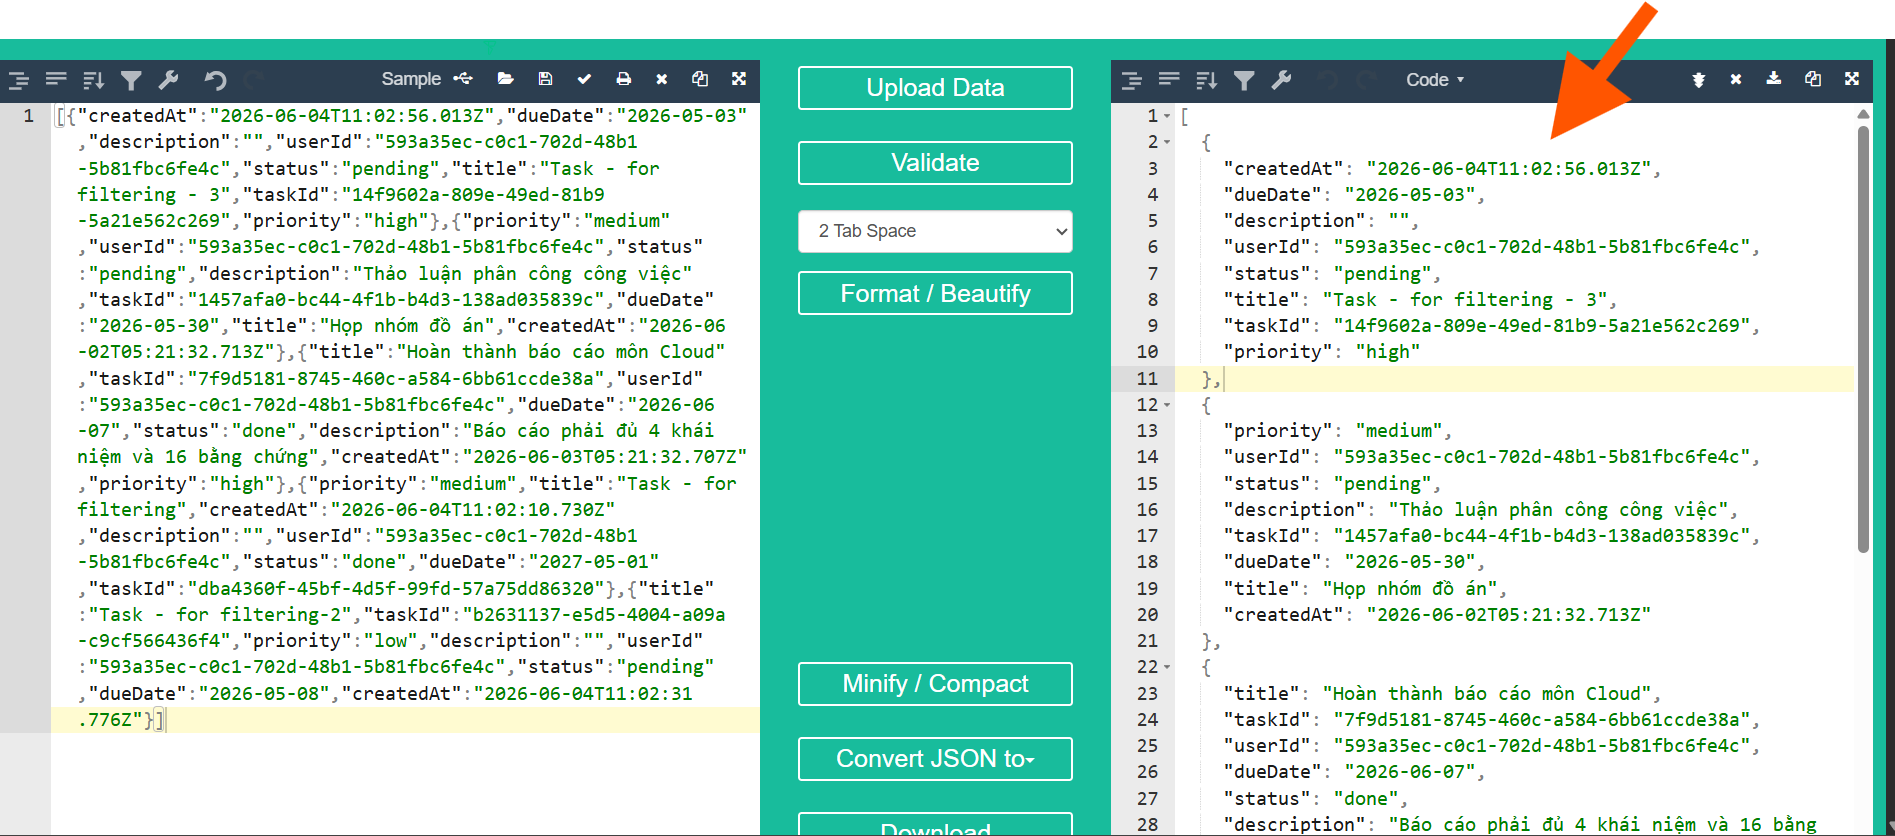
\includegraphics[width=0.8\textwidth]{image/CO-4.1.png}
    \caption{CO-4: Gọi API kèm Token hợp lệ trả về dữ liệu}
    \label{img:CO-4.1}
\end{figure}

%% ==================== PHẦN 3 ====================
\section{Kiến trúc Mạng, IAM và Giám sát Hệ thống}

\subsection{Kiến trúc Mạng — Custom VPC}
Toàn bộ hạ tầng compute được triển khai bên trong một Custom VPC.

\begin{itemize}
    \item \textbf{Private Subnets:} \texttt{TaskManager-Private-1a} và \texttt{TaskManager-Private-1b} ở hai AZ khác nhau (High Availability).
    \item \textbf{VPC Gateway Endpoint:} \texttt{TaskManager-DynamoDB-Endpoint}. Cho phép Lambda kết nối DynamoDB qua mạng riêng AWS.
    \item \textbf{Security Group:} Cấu hình deny-by-default, chỉ cho phép Outbound HTTPS (443) tới DynamoDB Prefix List. Không có đường ra internet công cộng (0.0.0.0/0).
\end{itemize}

\begin{figure}[H]
    \centering
    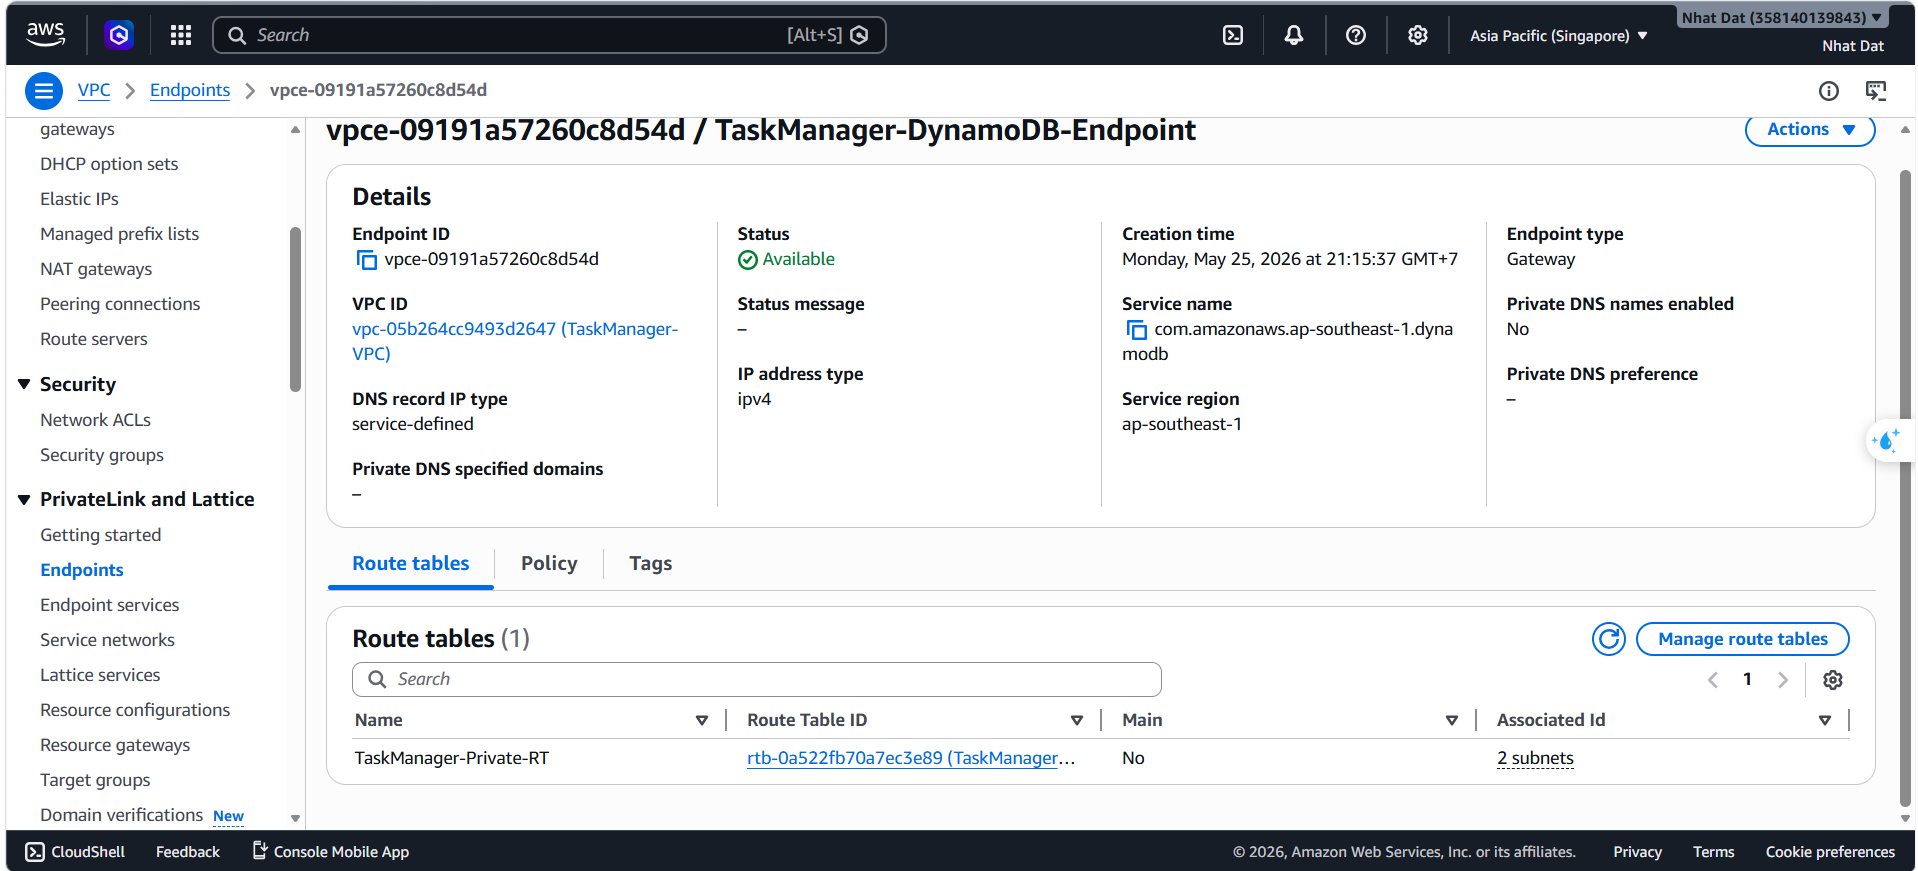
\includegraphics[width=0.8\textwidth]{image/NE-1.png}
    \caption{NE-1: VPC Gateway Endpoint cho DynamoDB (Status: Available)}
    \label{img:NE-1}
\end{figure}

\begin{figure}[H]
    \centering
    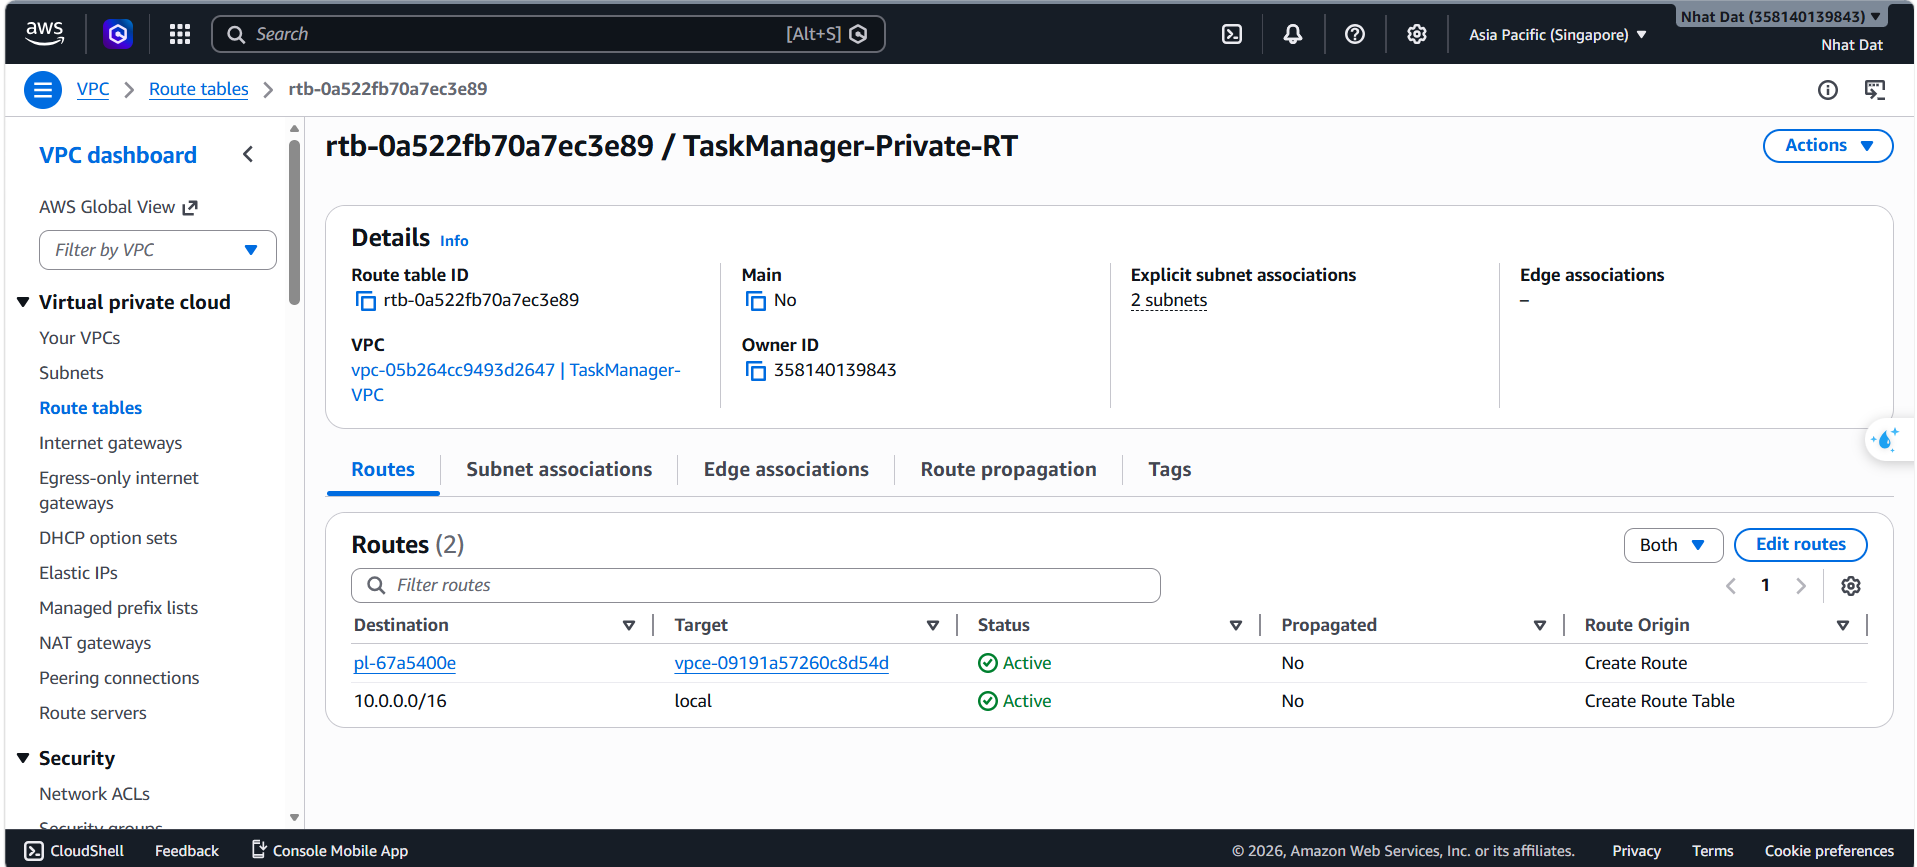
\includegraphics[width=0.8\textwidth]{image/NE-3.png}
    \caption{NE-3: Route Table điều hướng traffic qua VPCE}
    \label{img:NE-3}
\end{figure}

\begin{figure}[H]
    \centering
    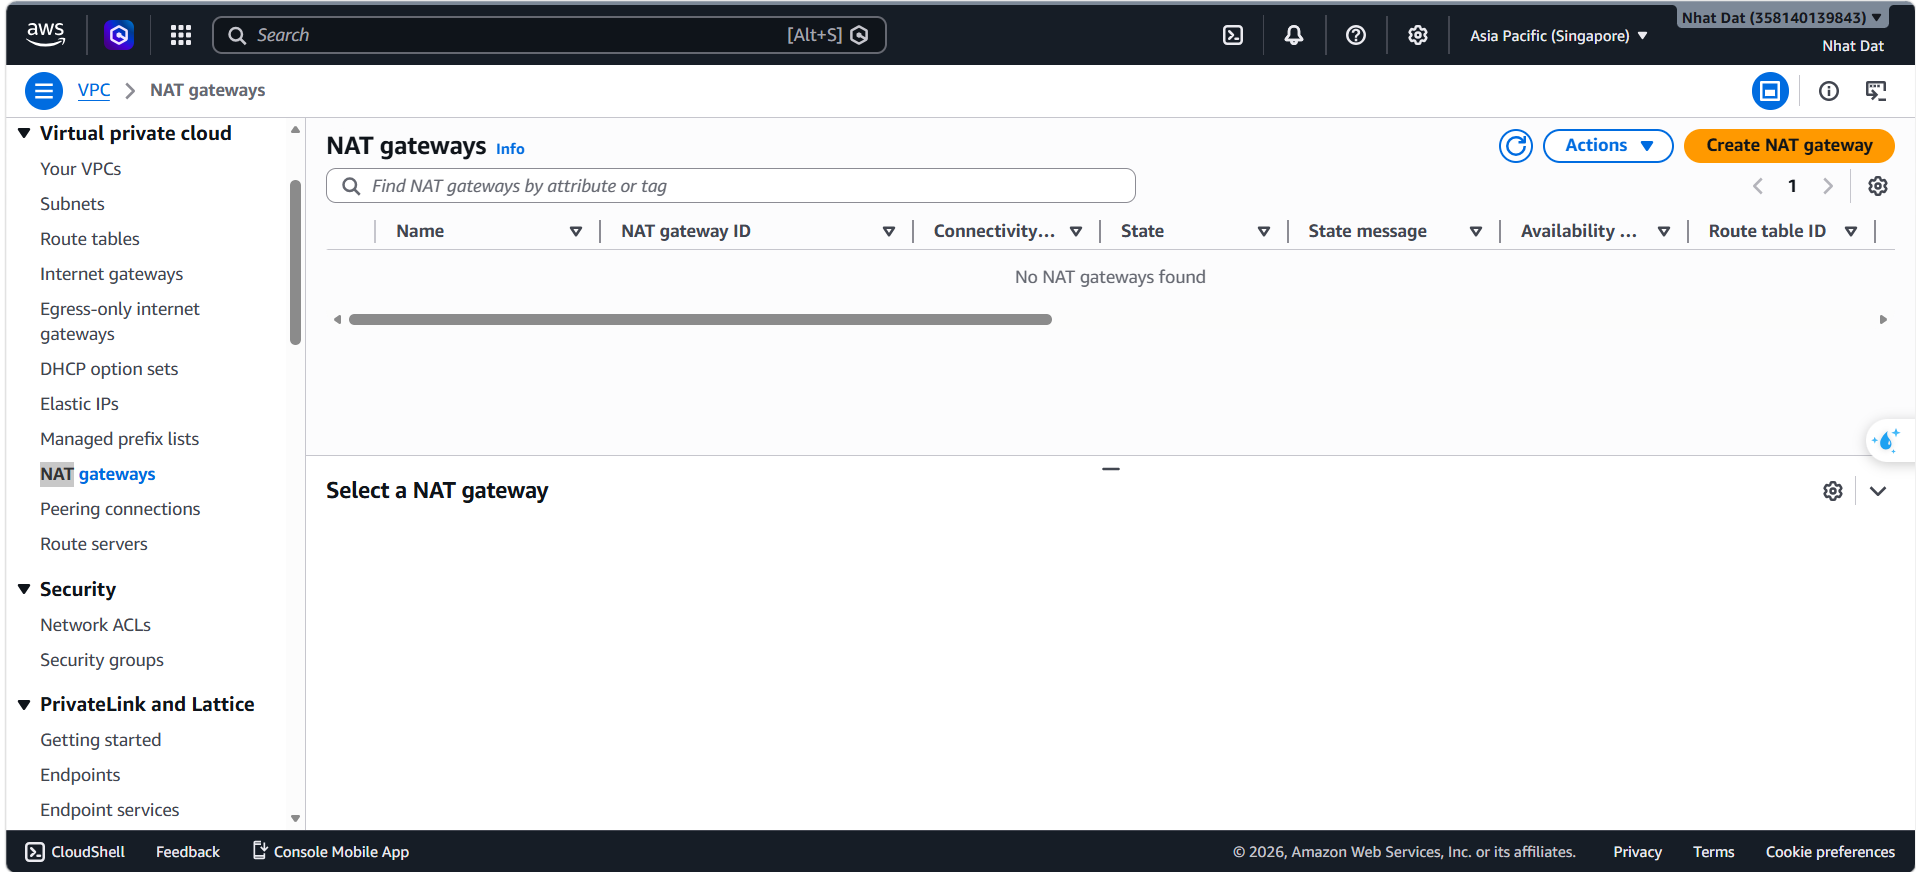
\includegraphics[width=0.8\textwidth]{image/NE-4.png}
    \caption{NE-4: Không sử dụng NAT Gateway}
    \label{img:NE-4}
\end{figure}

\subsection{Bảo mật IAM — Least Privilege}
Nhóm đã tạo 4 IAM Roles riêng biệt cho 4 Lambda functions để đảm bảo nguyên tắc Đặc quyền tối thiểu (Least Privilege).

\begin{figure}[H]
    \centering
    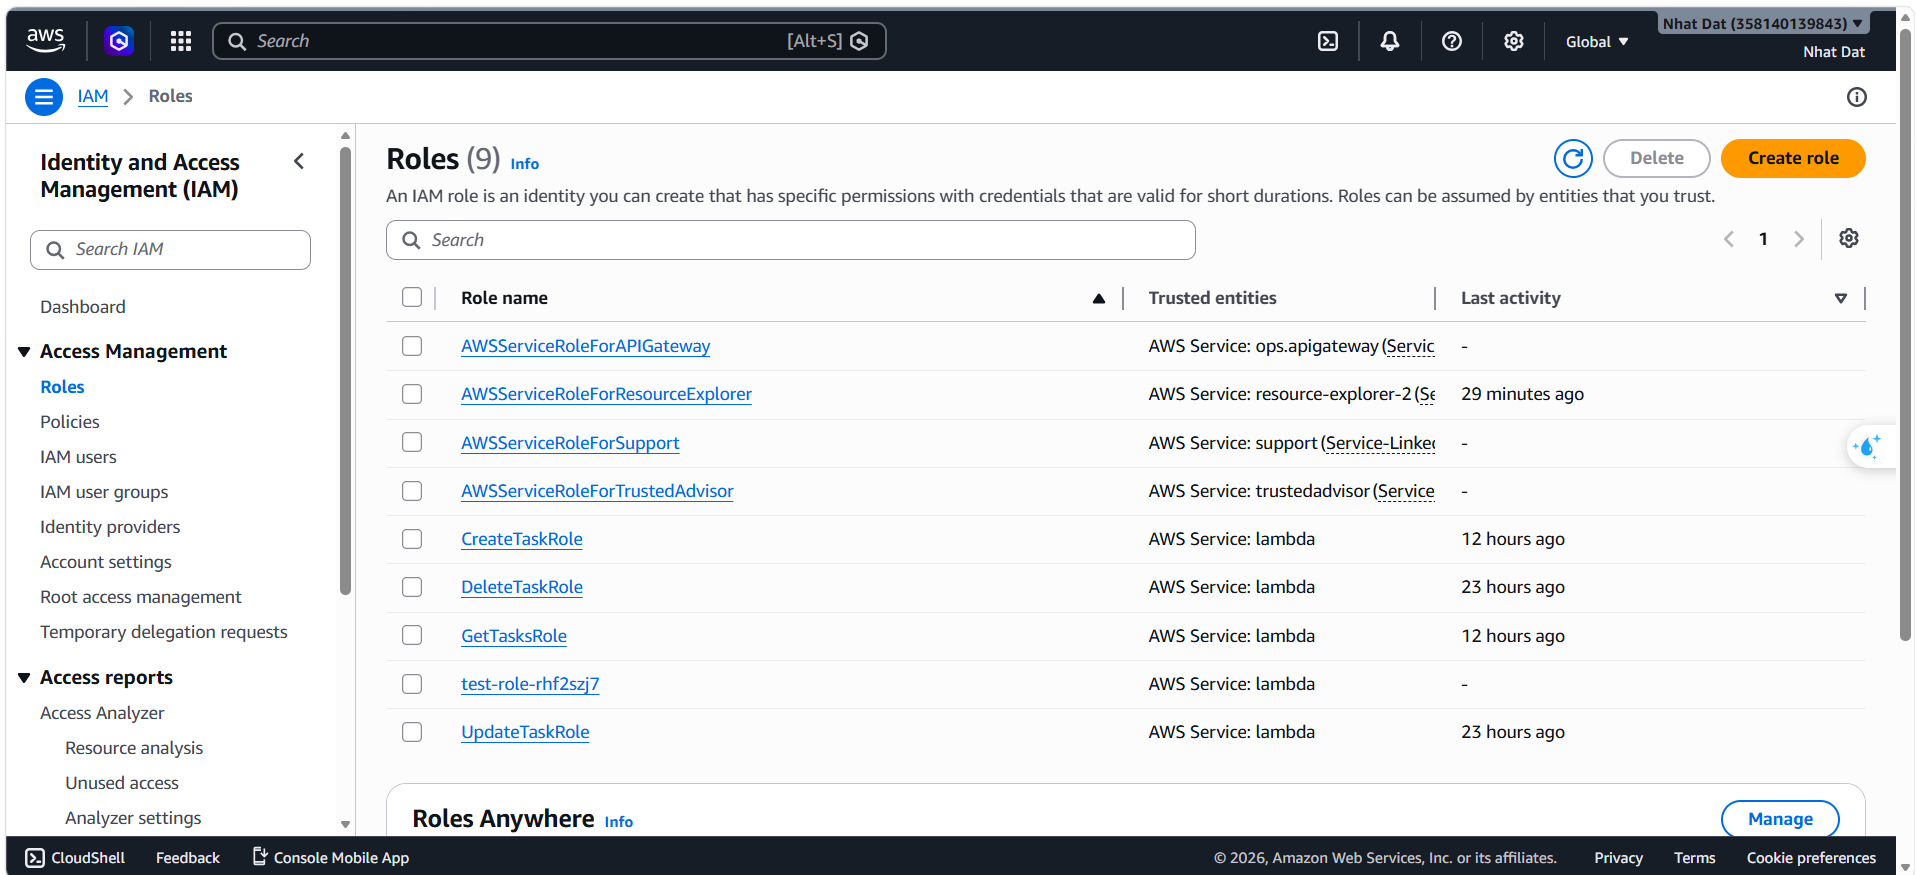
\includegraphics[width=0.8\textwidth]{image/IM-1.png}
    \caption{IM-1: Các IAM Roles phân biệt rõ ràng}
    \label{img:IM-1}
\end{figure}

Mỗi Role chỉ được cấp quyền thực hiện các API cụ thể (VD: chỉ \texttt{dynamodb:Query}) và giới hạn tài nguyên ở mức ARN của bảng cụ thể.

\begin{figure}[H]
    \centering
    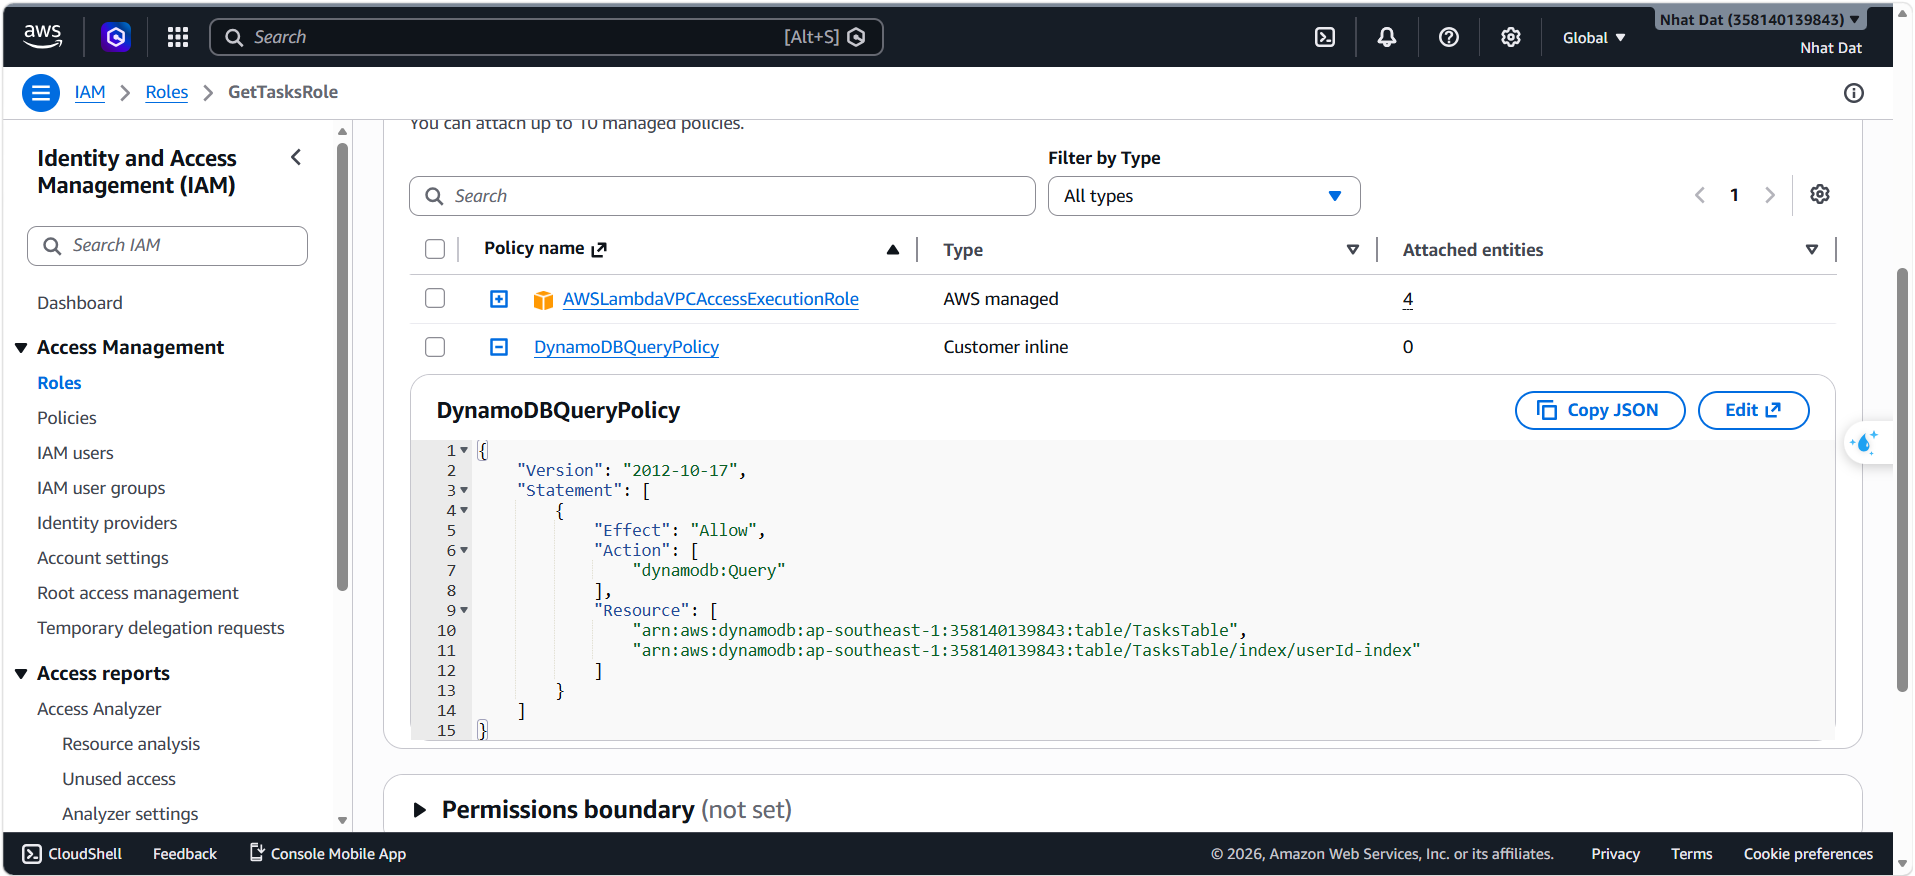
\includegraphics[width=0.8\textwidth]{image/IM-2.1.png}
    \caption{IM-2: Policy giới hạn quyền Query trên ARN cụ thể}
    \label{img:IM-2.1}
\end{figure}

\begin{figure}[H]
    \centering
    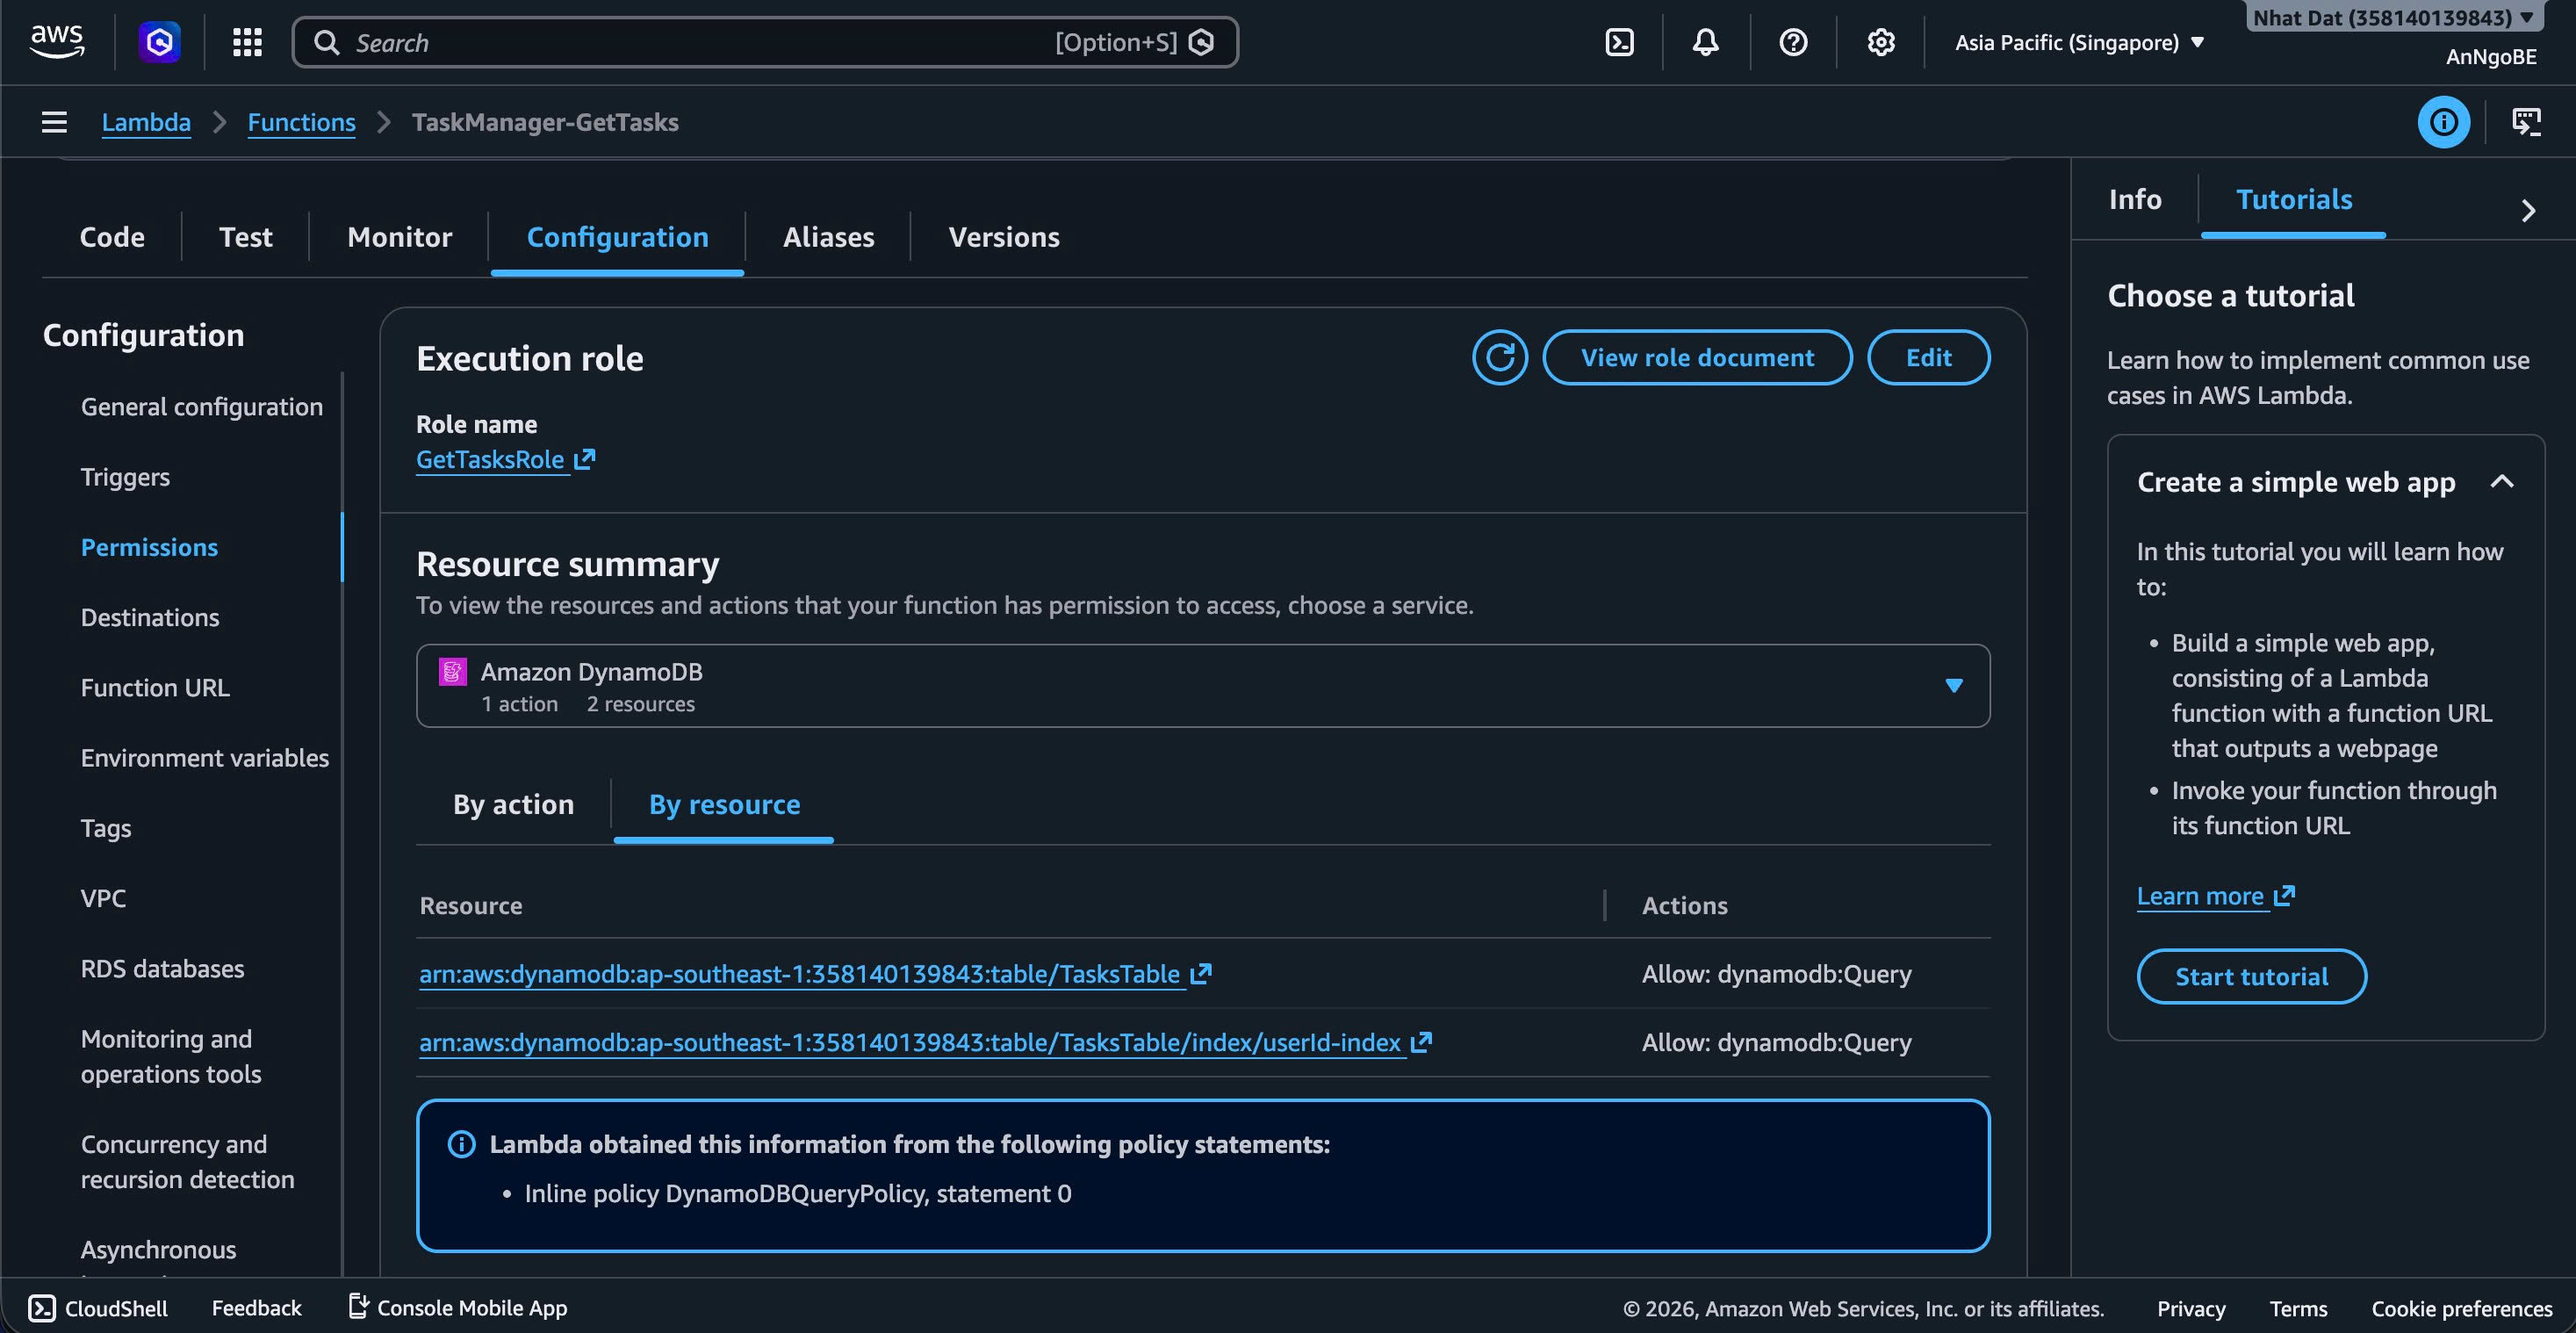
\includegraphics[width=0.8\textwidth]{image/IM-3.1.jpg}
    \caption{IM-3: Lambda GetTasks được gắn Role tương ứng}
    \label{img:IM-3.1}
\end{figure}

\subsection{Hệ thống Giám sát — CloudWatch \& SNS}
Dashboard được thiết lập với 6 widgets giám sát thời gian thực: số lần gọi Lambda, thời lượng chạy, lỗi, và độ trễ API. Đồng thời thiết lập 2 CloudWatch Alarms để gửi email cảnh báo qua SNS khi có lỗi.

\begin{figure}[H]
    \centering
    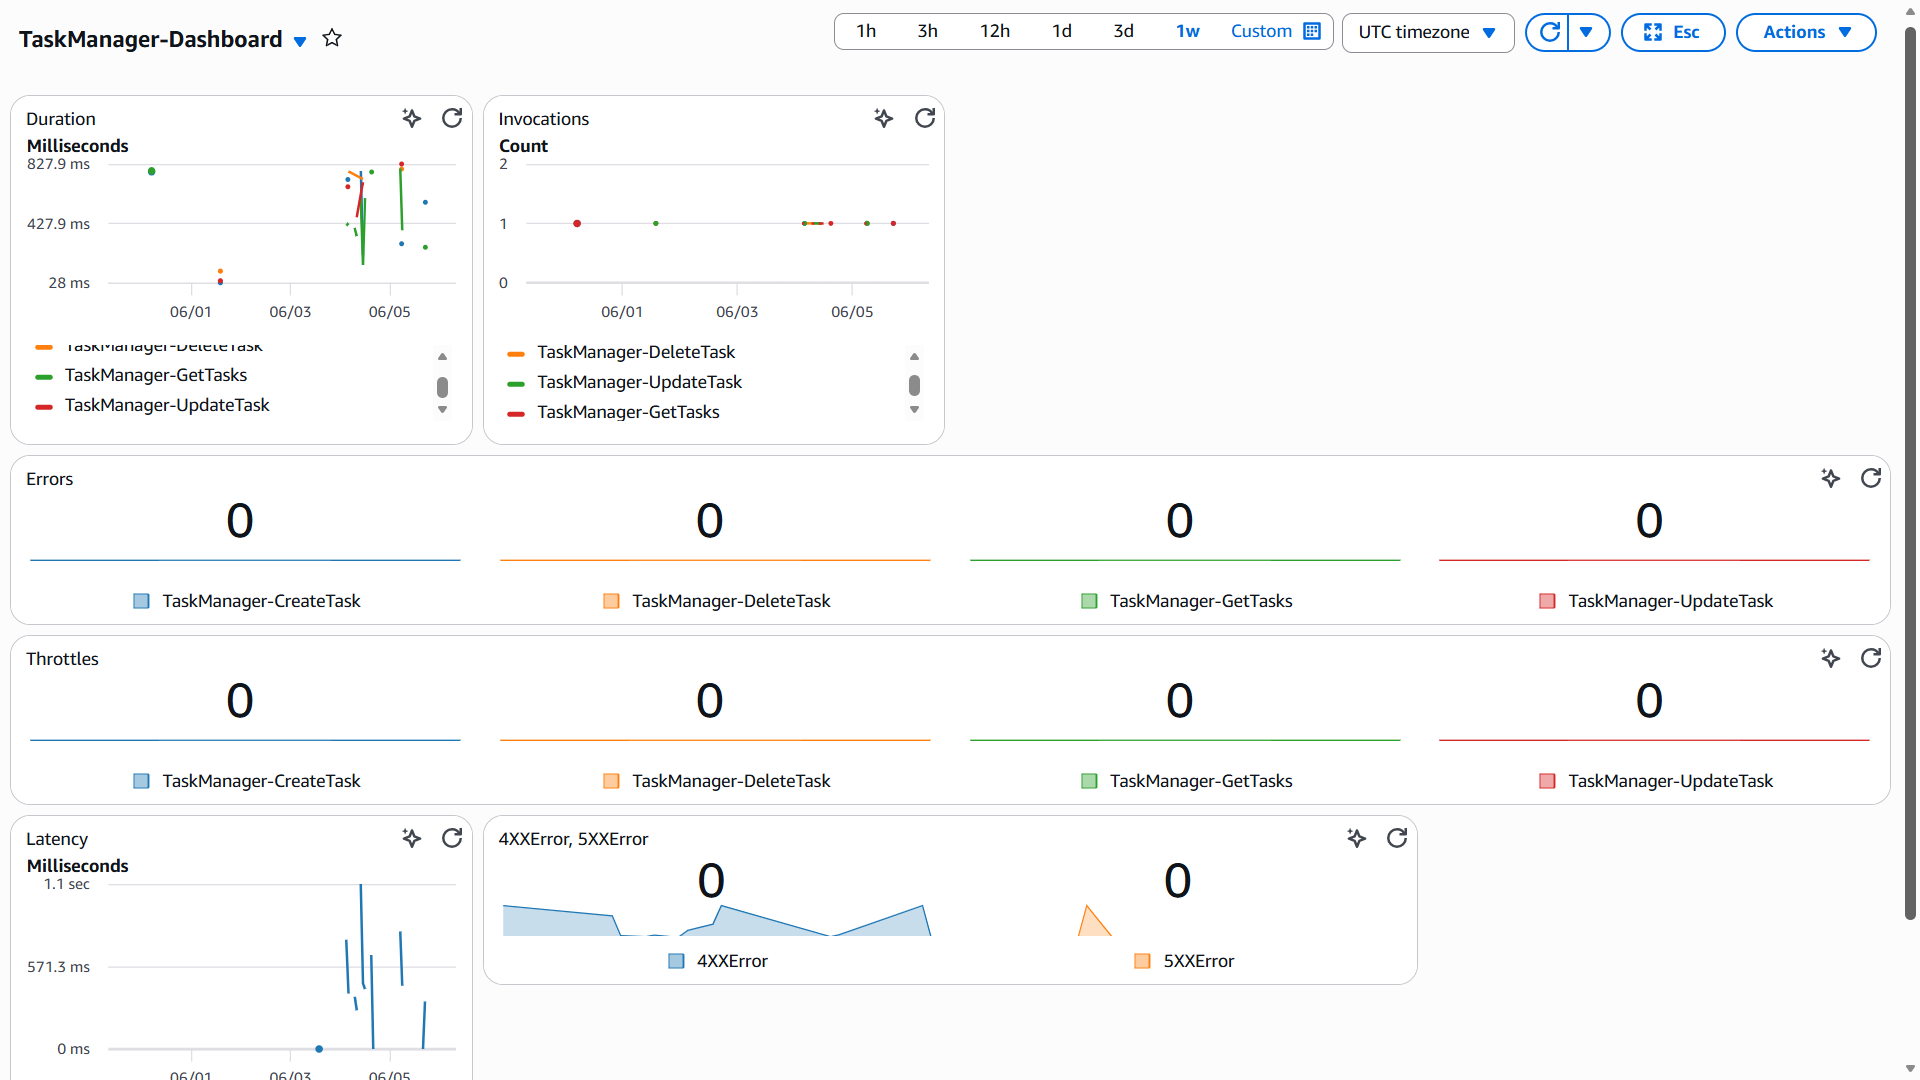
\includegraphics[width=0.8\textwidth]{image/DB-1.png}
    \caption{DB-1: CloudWatch Dashboard}
    \label{img:DB-1}
\end{figure}

\begin{figure}[H]
    \centering
    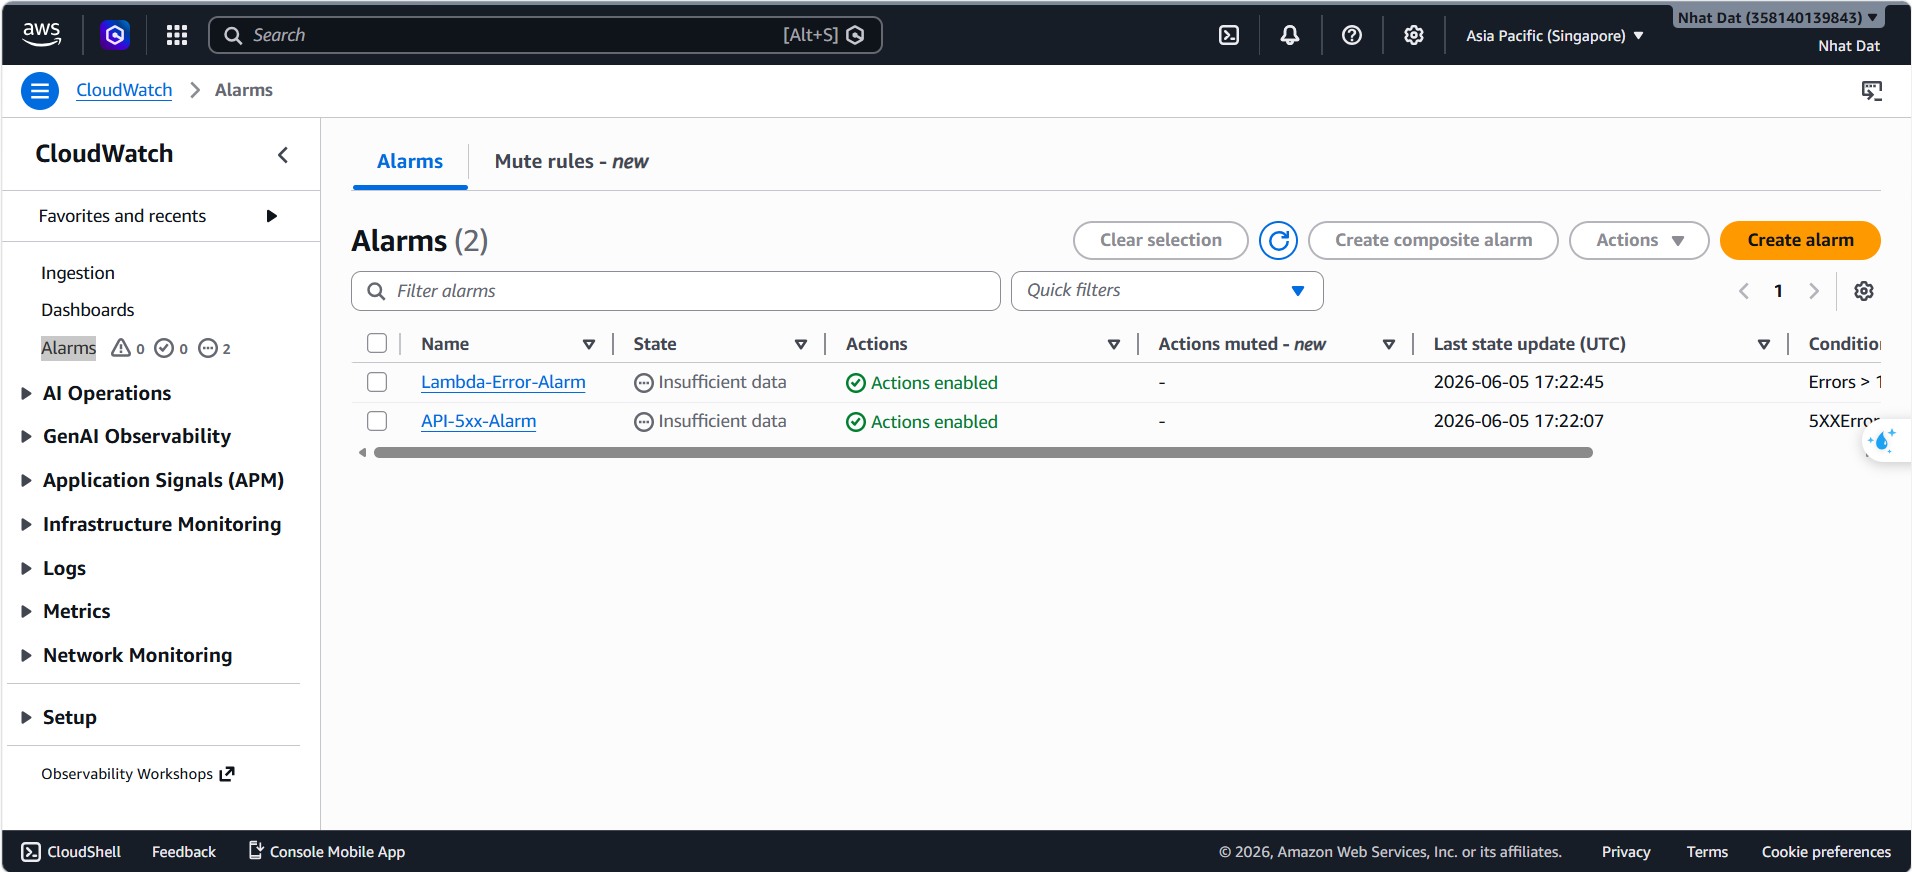
\includegraphics[width=0.8\textwidth]{image/CW-1.png}
    \caption{CW-1: Các CloudWatch Alarms giám sát lỗi}
    \label{img:CW-1}
\end{figure}

\begin{figure}[H]
    \centering
    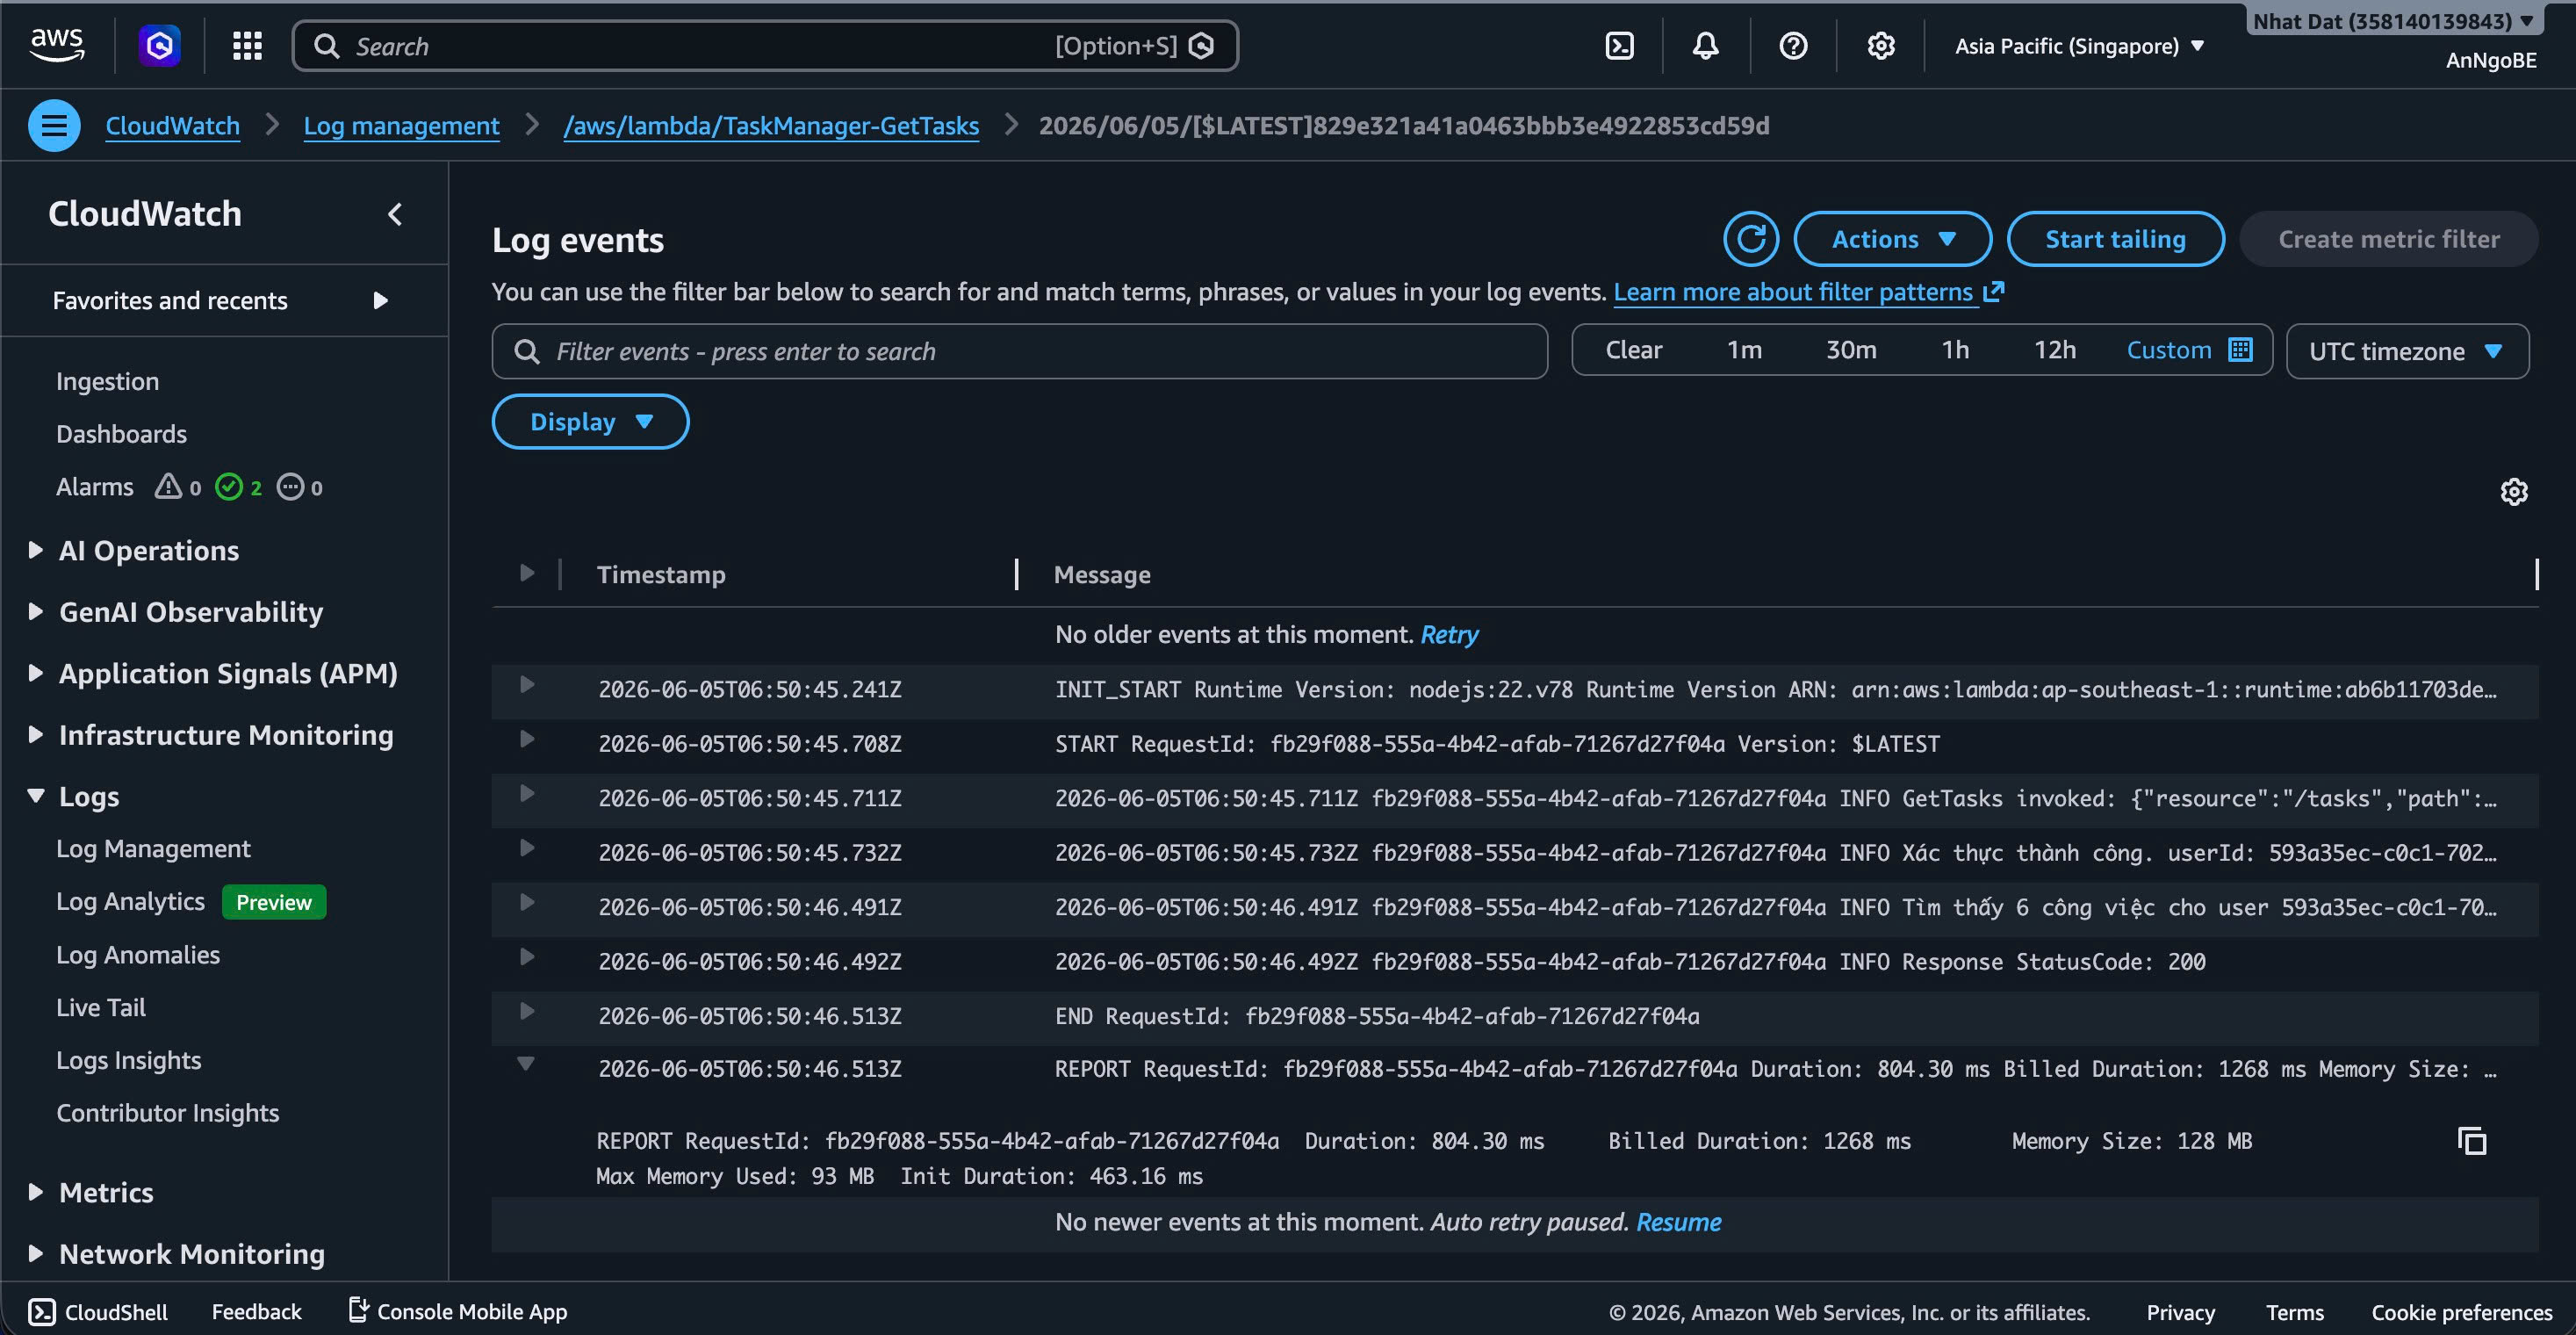
\includegraphics[width=0.8\textwidth]{image/NE-5.1.jpg}
    \caption{NE-5: Log CloudWatch chứng minh Lambda gọi DynamoDB thành công}
    \label{img:NE-5.1}
\end{figure}

\subsection{Kiểm soát và Tối ưu Chi phí}
Thiết lập AWS Budget ở mức giới hạn \$0.01, với hai mốc cảnh báo (80\% và 100\%) gửi qua email. Toàn bộ hệ thống tận dụng tối đa Serverless và Free Tier, không sử dụng NAT Gateway hay ALB, giúp chi phí thực tế duy trì ở mức \$0.

\begin{figure}[H]
    \centering
    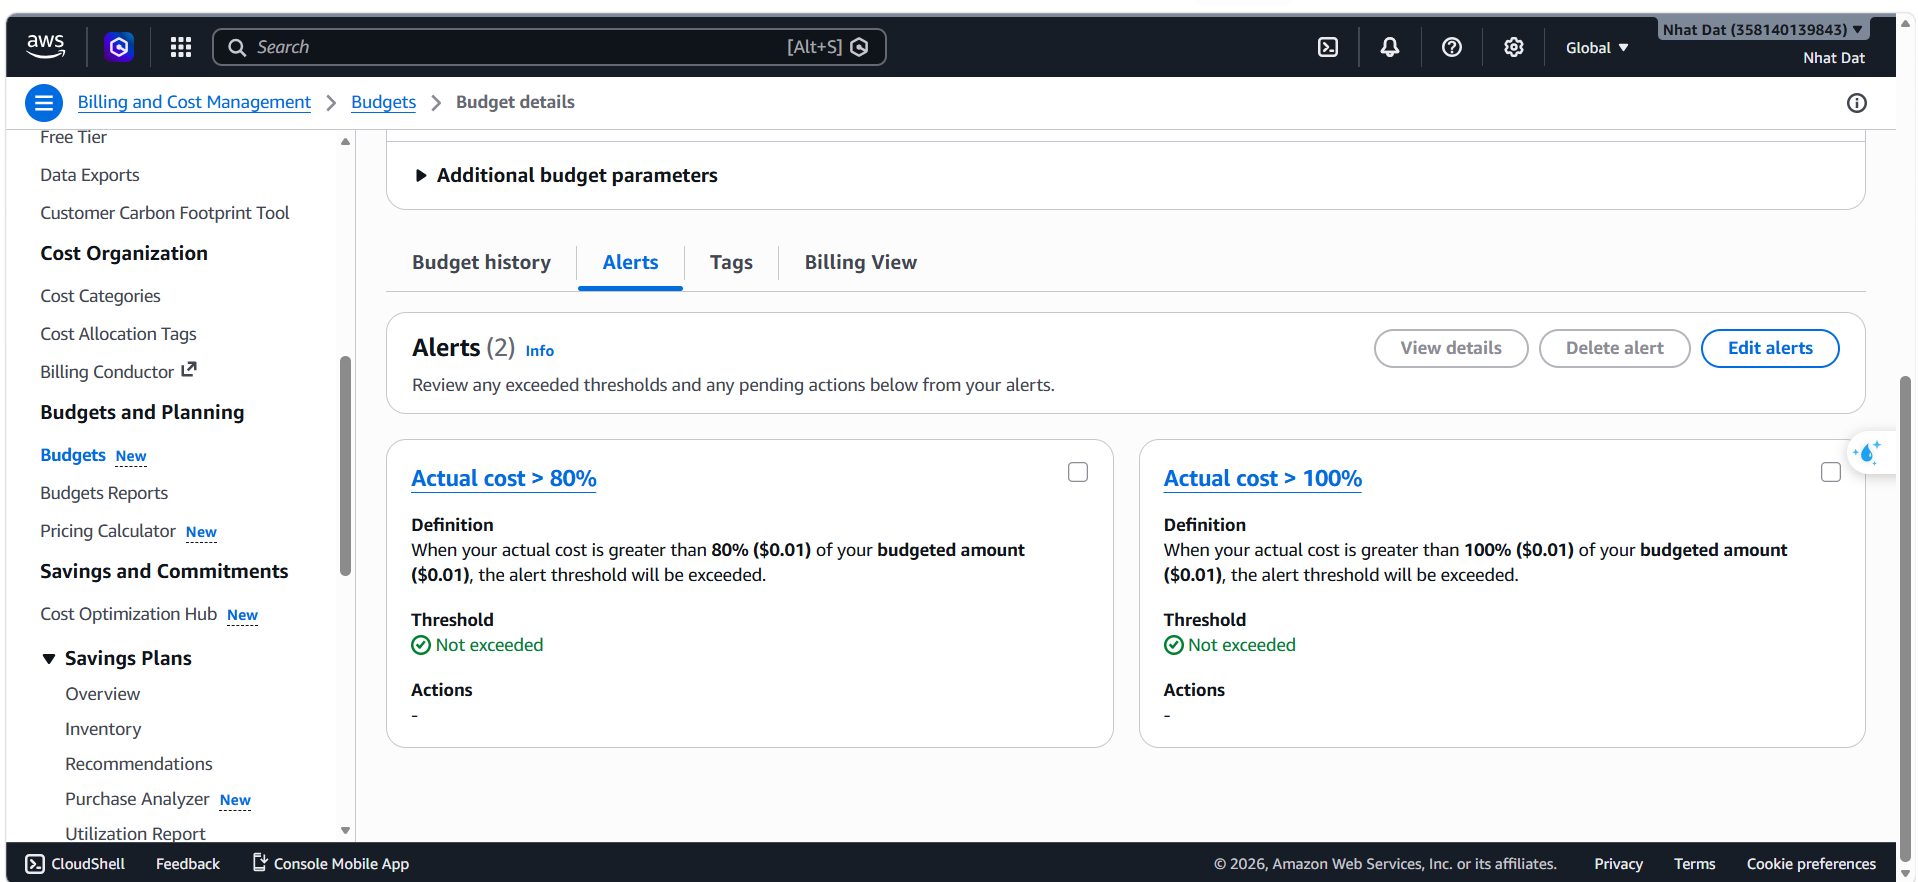
\includegraphics[width=0.8\textwidth]{image/BG-1.png}
    \caption{BG-1: Cấu hình AWS Budget}
    \label{img:BG-1}
\end{figure}

\begin{figure}[H]
    \centering
    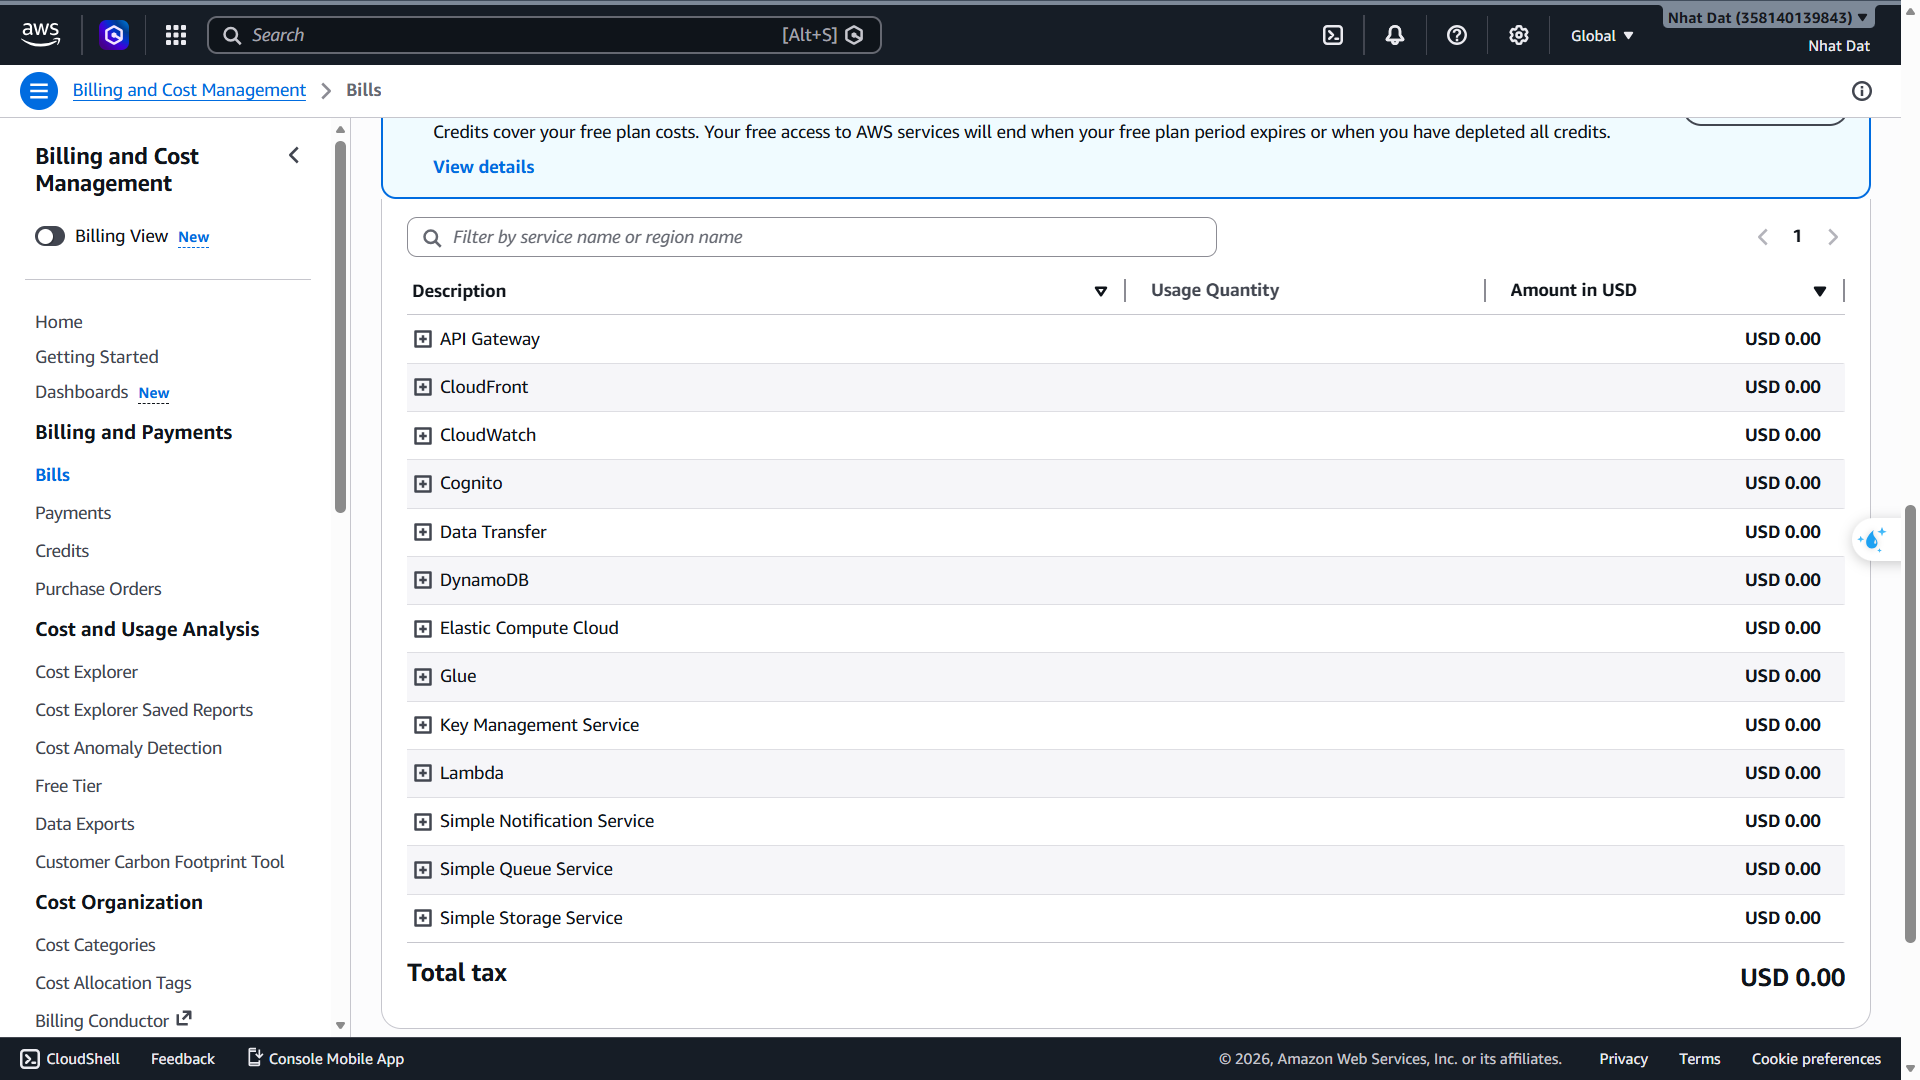
\includegraphics[width=0.8\textwidth]{image/CS-1.png}
    \caption{CS-1: Báo cáo chi phí (Cost Explorer) bằng \$0}
    \label{img:CS-1}
\end{figure}

%% ==================== PHẦN 4 ====================
\section{Giải thích Các Khái niệm Kỹ thuật Cốt lõi}

\subsection{Luồng đi của Request}
Khi người dùng tạo công việc mới:
\begin{enumerate}
    \item Trình duyệt gửi POST request kèm JWT Token tới API Gateway.
    \item API Gateway kiểm tra Throttling và xác minh Cognito Token (qua Authorizer).
    \item Nếu hợp lệ, API Gateway kích hoạt Lambda \texttt{CreateTask} nằm trong Private Subnet.
    \item Lambda xử lý logic, tạo dữ liệu mới và gửi lệnh \texttt{PutItem} qua mạng riêng AWS thông qua VPC Gateway Endpoint.
    \item Traffic tới DynamoDB mà không đi qua Internet.
    \item Kết quả trả về theo đường ngược lại để đến trình duyệt.
\end{enumerate}

\begin{figure}[H]
    \centering
    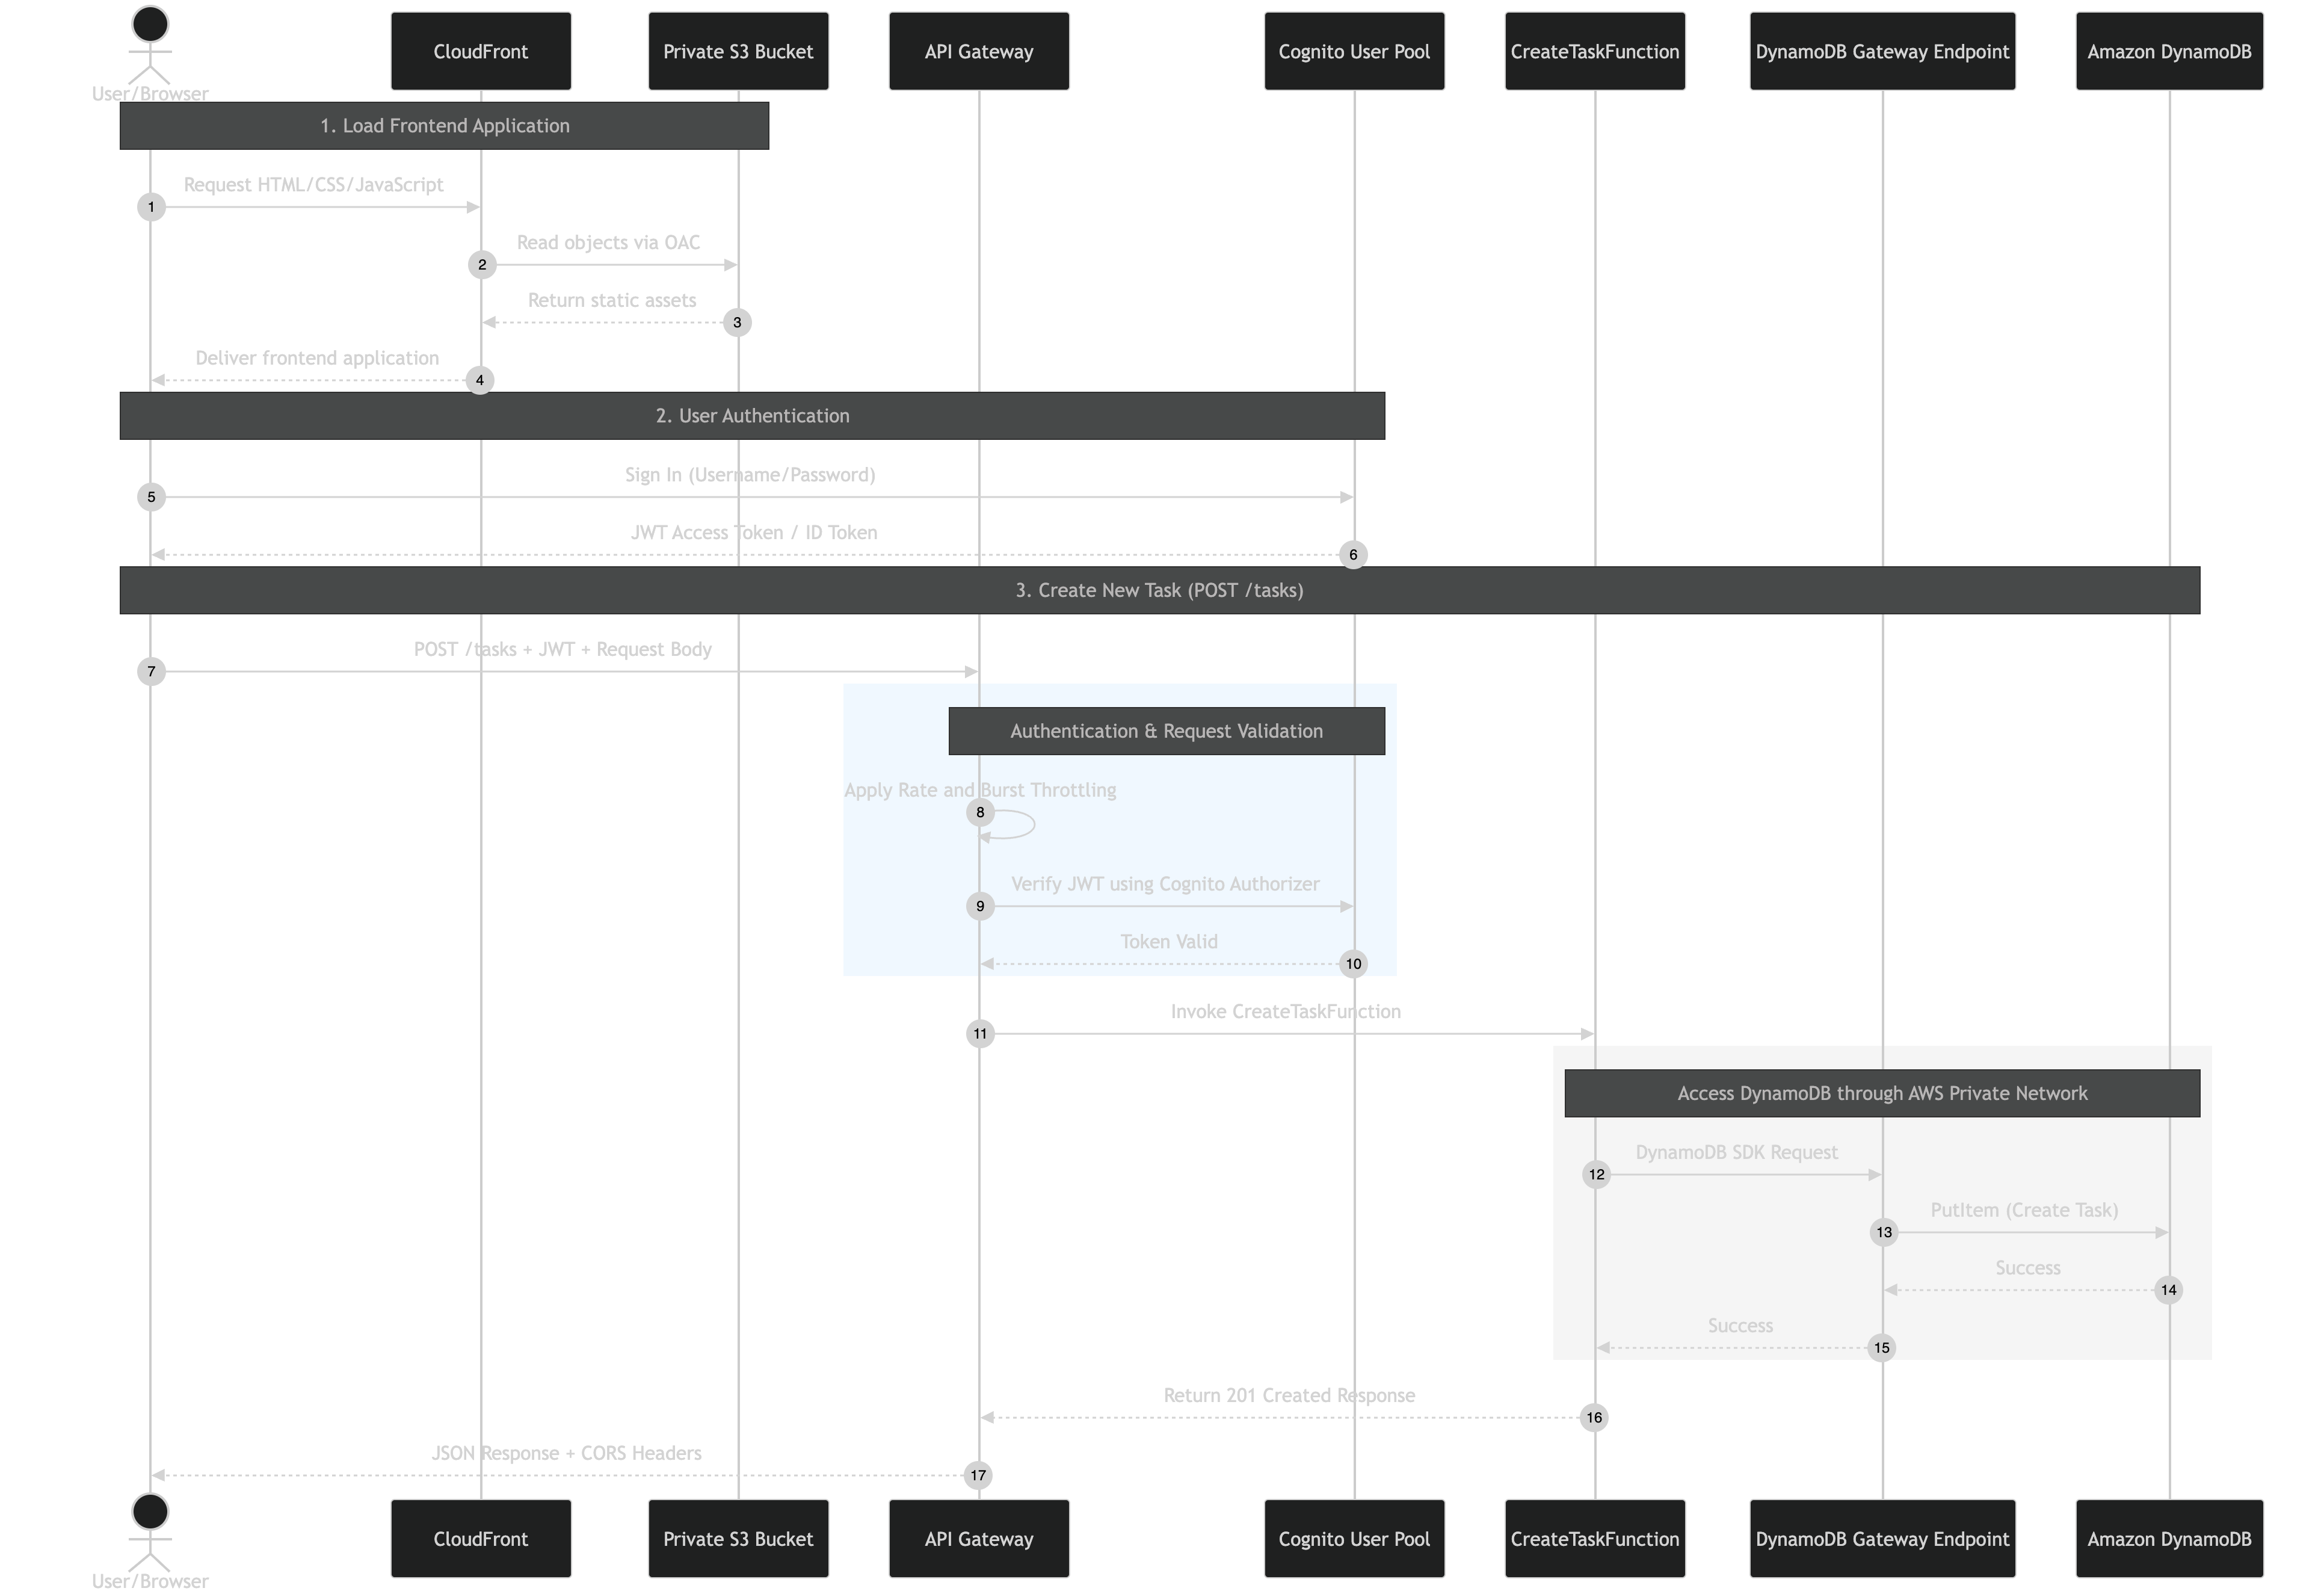
\includegraphics[width=0.8\textwidth]{image/SD-3.png}
    \caption{SD-3: Sơ đồ tuần tự minh họa luồng Request}
    \label{img:SD-3}
\end{figure}

\subsection{VPC Gateway Endpoint so với NAT Gateway}
\begin{itemize}
    \item \textbf{VPC Gateway Endpoint (Đang dùng):} Traffic từ Lambda tới DynamoDB đi trên mạng backbone riêng của AWS. Hoàn toàn miễn phí (\$0) và bảo mật hơn vì không ra internet.
    \item \textbf{NAT Gateway (Không dùng):} Phải cấu hình qua Internet Gateway. Chi phí rất cao (\textasciitilde\$32/tháng) và có rủi ro bảo mật vì dữ liệu đi qua internet công cộng.
\end{itemize}

\begin{figure}[H]
    \centering
    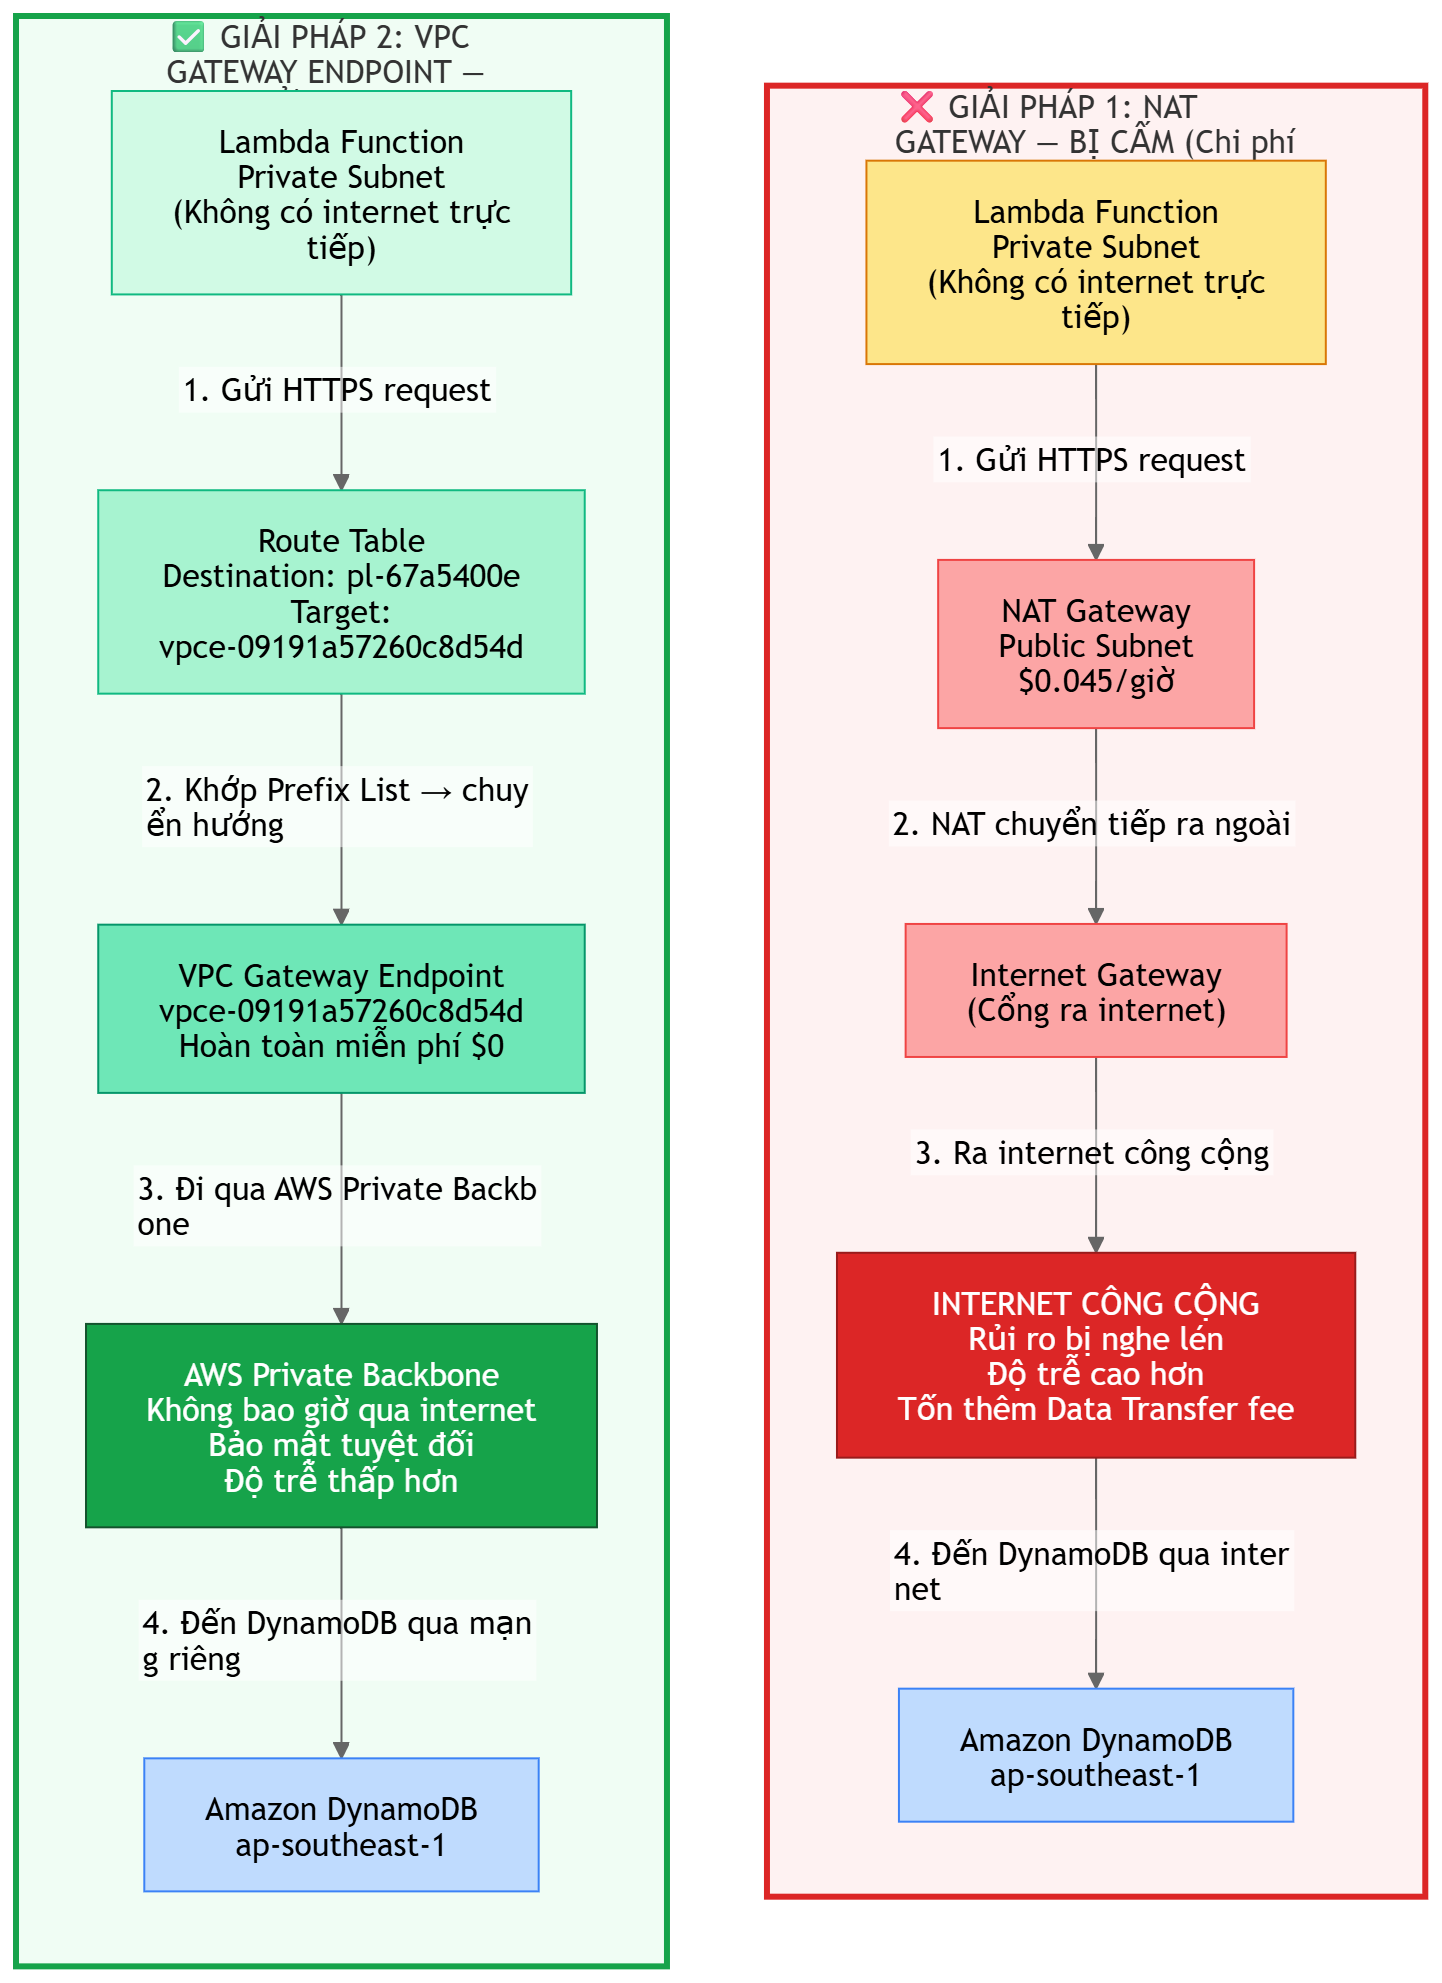
\includegraphics[width=0.8\textwidth]{image/SD-1.png}
    \caption{SD-1: Sơ đồ so sánh VPC Gateway Endpoint và NAT Gateway}
    \label{img:SD-1}
\end{figure}

\subsection{Khả năng Tự động Mở rộng (Auto Scaling)}
Kiến trúc hoàn toàn Serverless theo mô hình "scale to zero":
\begin{itemize}
    \item \textbf{Lambda:} Không có request $\rightarrow$ không có máy chủ nào chạy. Khi có nhiều request, Lambda tự động khởi tạo nhiều instances song song (tối đa theo hạn mức).
    \item \textbf{API Gateway:} Tự động đóng vai trò như Load Balancer, phân phối tải tới các Lambda instances mà không cần máy chủ cân bằng tải (ALB) truyền thống.
\end{itemize}

\subsection{Sơ đồ Kiến trúc Tổng thể}
\begin{figure}[H]
    \centering
    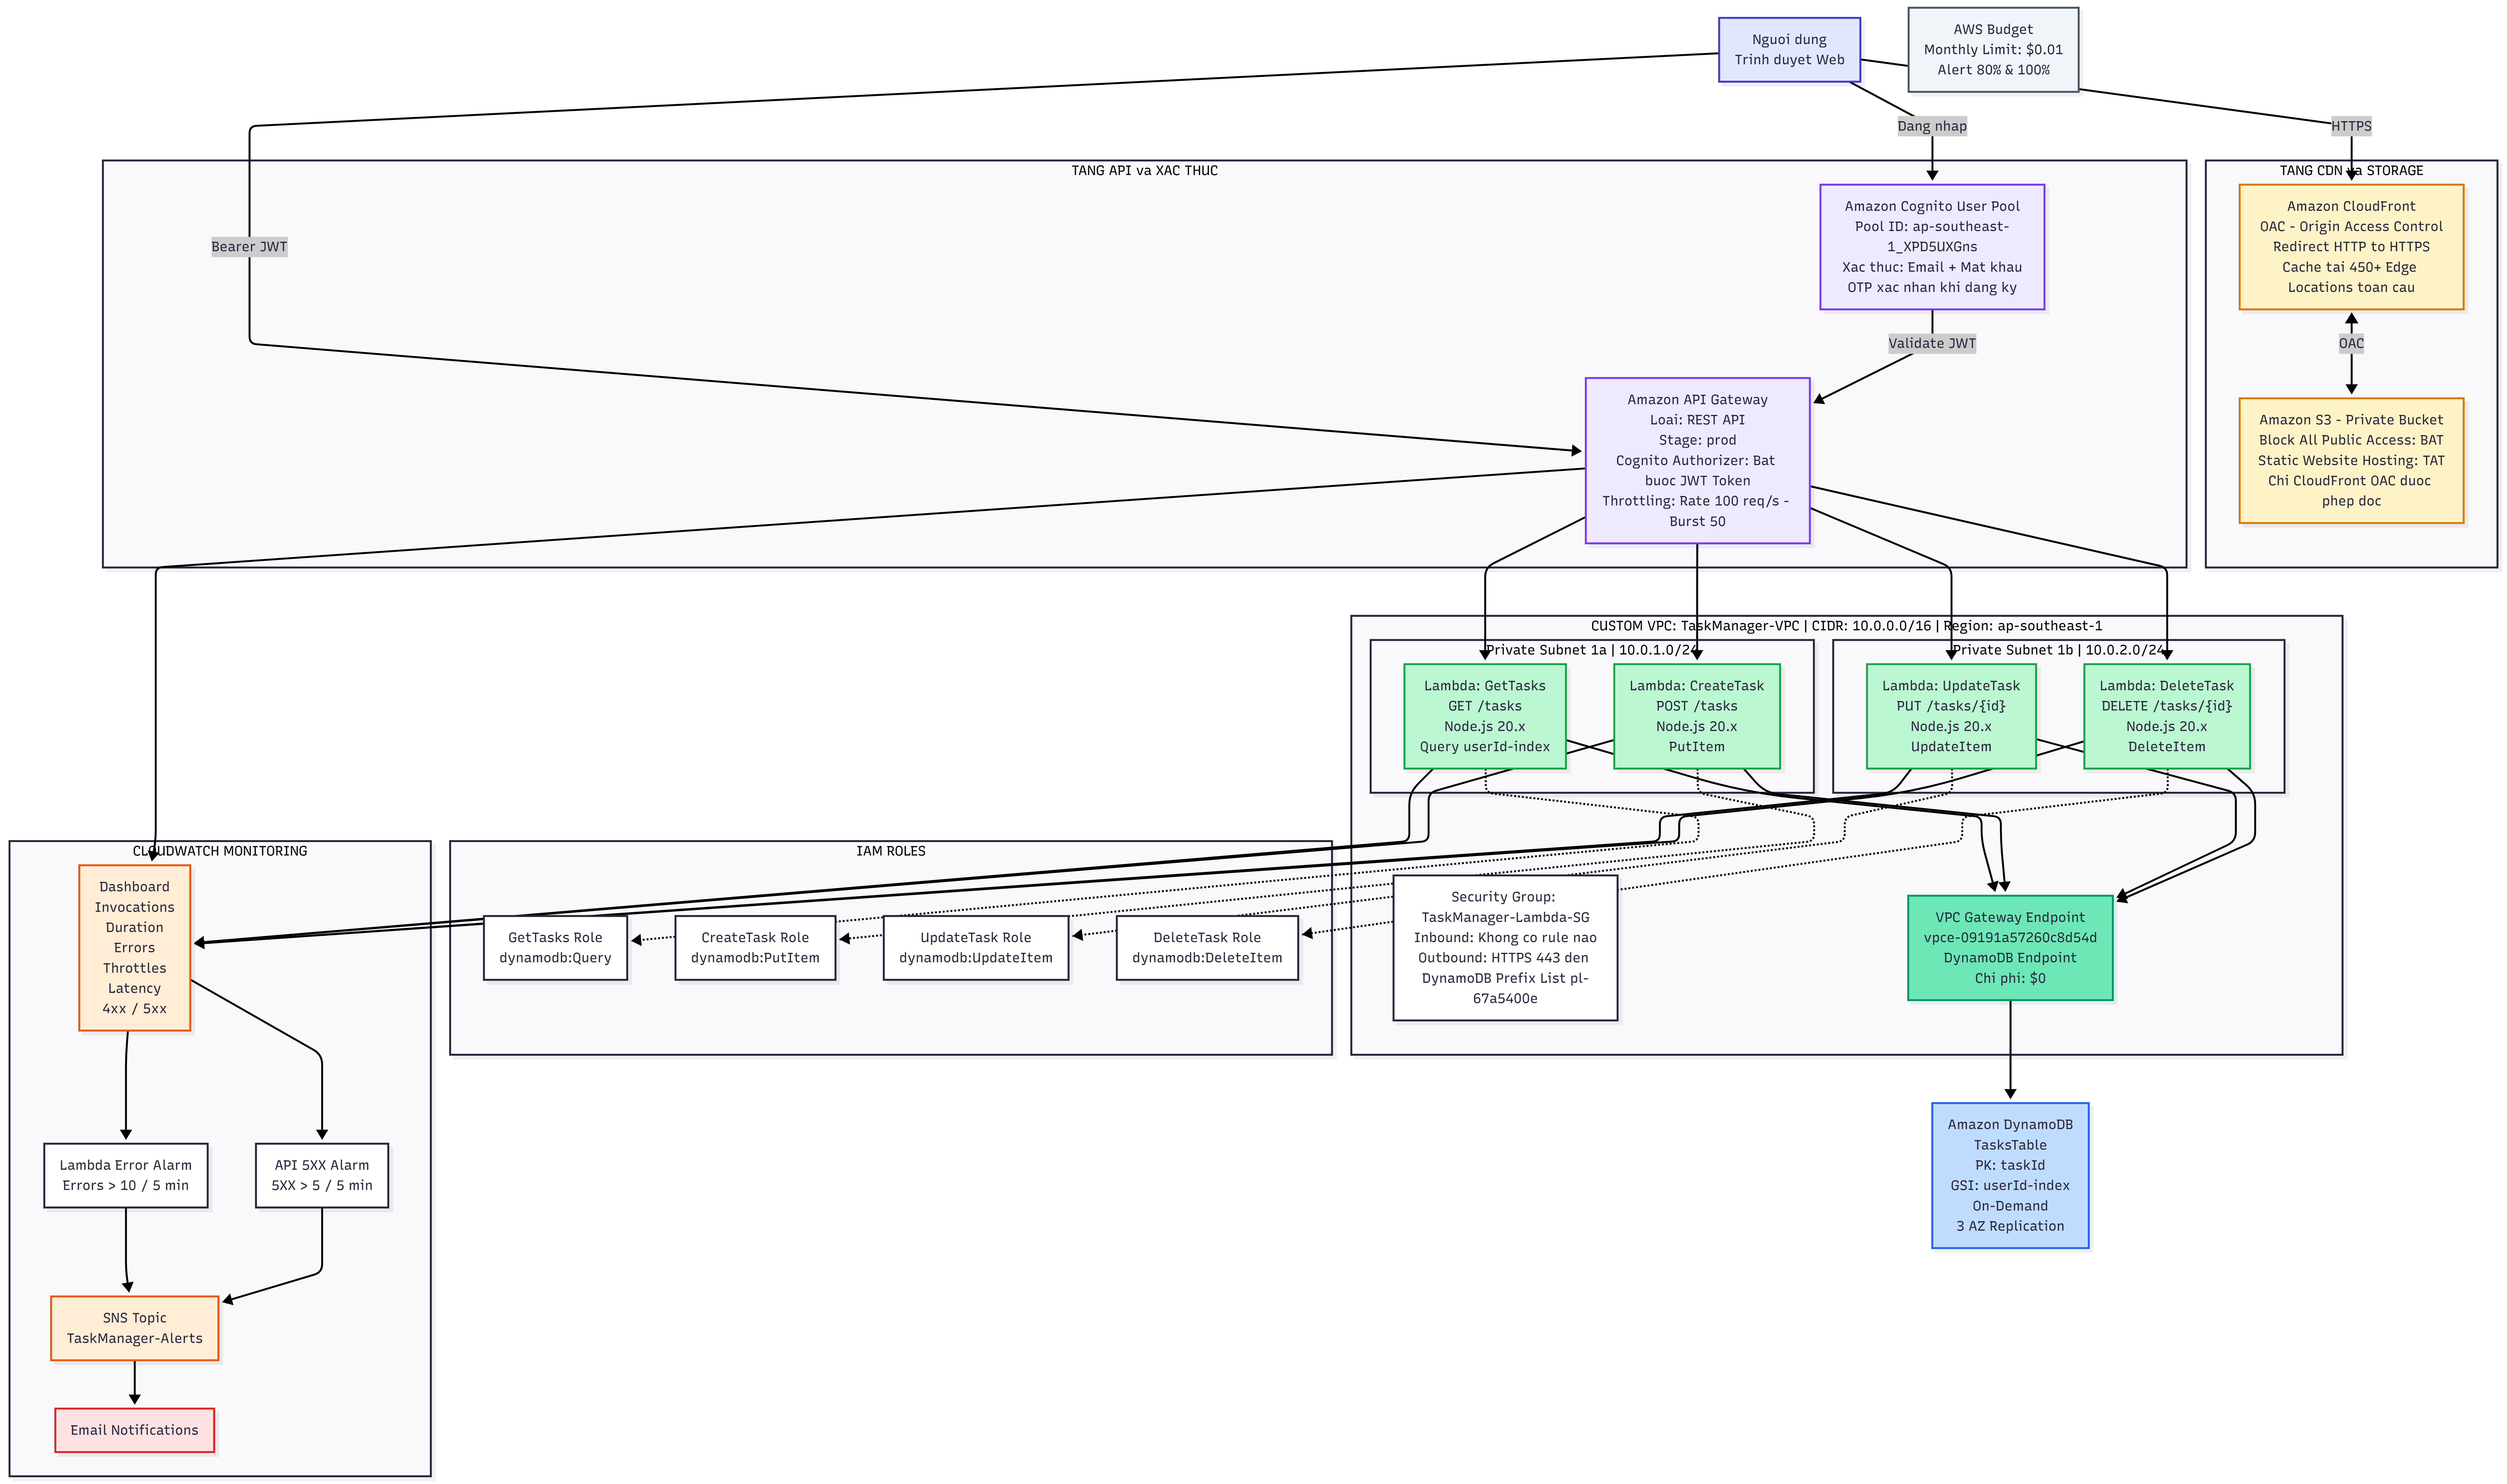
\includegraphics[width=1\textwidth]{image/SD-2.png}
    \caption{SD-2: Sơ đồ kiến trúc Serverless hệ thống}
    \label{img:SD-2}
\end{figure}



%% ==================== PHẦN 6 ====================
\section{Lịch sử Sử dụng AI}
\textit{[Mục này sẽ được bổ sung sau theo lịch sử Prompt AI của thành viên khác]}

%% ==================== PHẦN 7 ====================
\newpage
\section{Tài liệu Tham khảo}
% Để trống theo yêu cầu

\end{document}
